\documentclass[hyperref={pdfpagelabels=false}]{beamer}
\usepackage{pgf}
\usepackage[utf8]{inputenc}
\usepackage{lmodern}
\usepackage{graphicx}          	% add graphics
\usepackage{tikz,pgfplots}
\usepackage{gincltex}
\usepackage{epstopdf}
\usepackage{enumerate}		% lists of items
\usepackage[linesnumbered,lined,boxed,ruled,commentsnumbered]{algorithm2e}
\usepackage{setspace}
\usepackage{listings}		% code listings
\usepackage[backend=biber,style=authortitle-comp]{biblatex}
\addbibresource{presentation.bib}

\usetheme{Dresden}
\setbeamerfont{subsection in toc}{size=\small}
\setbeamertemplate{blocks}[rounded][shadow=false]


\title{Scaling Geometric Monitoring Over Distributed Streams}  
\author{Alexandros D. Keros} 
\date{June 23, 2016} 
\addtobeamertemplate{title page}{}{\begin{center}\small Supervised by: Prof. V.Samoladas\end{center}}

\begin{document}

\begin{frame}
\titlepage
\end{frame} 


\begin{frame}
\frametitle{Table of contents}
\tableofcontents
\end{frame} 

%%%%%%%%%%%%%  section: INTRODUCTION  %%%%%%%%%%%%%%%%%%%%%%%
\section{Introduction}
\begin{frame}
  \tableofcontents[currentsection]
 \end{frame}
 
\subsection*{Overview}
\begin{frame} \frametitle{Data Stream Systems}\framesubtitle{\tiny(\fullcite{Babcock2002DataStreamSystems})}
\begin{itemize}
\item \textbf{Data streams}: Continuous, high volume, size unbound, violative, probably distributed
\item \emph{Pull paradigm}
\item Centralizing and/or polling $\rightarrow$ prohibitive in terms of communication overhead
\item Examples: telecommunication, sensor networks 
\end{itemize}
\end{frame}

\begin{frame} \frametitle{The Geometric Monitoring Method}\framesubtitle{\tiny(\fullcite{Sharfman2006GM})}
\begin{itemize}
\item Threshold monitoring
\item Nodes communicate when needed
	\begin{itemize}
	\item Local constraints
	\item Violation resolution (\emph{false alarms})
	\end{itemize}
\item Arbitrary function monitoring
\item Tight accuracy bounds
\item A promising framework for \emph{distributed data stream monitoring}
\end{itemize}
\end{frame}

\begin{frame} \frametitle{Motivation}
\setbeamercovered{transparent}
\begin{itemize}
\item[]<1-> Problems:
\begin{itemize}
	\item<1-> increasing node population
	\item<1-> data volume
	\item<1-> data dimensionality
	\item<1-> arbitrary functions
	\item<2-> \textbf{communication - accuracy tradeoff}
\end{itemize}
\item[]<3->Need for:
\begin{itemize}
	\item<3-> scalability warranties
	\item<3-> tight accuracy bounds
	\item<3-> incremental/real-time operation
	\item<4-> \textbf{Minimize communication while retaining accuracy bounds}
\end{itemize}
\end{itemize}
\end{frame}

\begin{frame} \frametitle{Contributions}
\setbeamercovered{transparent}
Expand the \emph{geometric monitoring method}:
\begin{itemize}
\item<1-> heuristic method for violation resolution
\item<2-> distance-based hierarchical node clustering \tiny(\fullcite{Keren2014GMHetStreams})
\item<3-> throughout method evaluation on synthetic and real-world datasets
\end{itemize}
\end{frame}

%%%%%%%%%%%%%  section: THEOR BACK  %%%%%%%%%%%%%%%%%%%%%%%
\section{Theoretical Background}
\begin{frame}
  \tableofcontents[currentsection]
 \end{frame}
\subsection{The Geometric Monitoring Method}
\begin{frame} \frametitle{Geometric Threshold Monitoring}
\begin{itemize}
\item \fullcite{Sharfman2006GM}
\item \textbf{Threshold monitoring}: arbitrary function $f(\cdot)$, threshold $T$\\
 $$f(\cdot)<T\ \text{or}\ f(\cdot)>T$$
\item \textbf{Idea}: decompose into local constraints at the nodes
\end{itemize}
\end{frame}

\begin{frame} \frametitle{System Architecture} \framesubtitle{Centralized Scenario}
\begin{figure}[H]
\centering
\vspace{-1cm}
\includegraphics[scale=0.5]{../img/centralized.tex}
\caption{\textbf{Star-like network topology} example of the centralized scenario.The bold node represents the coordinator node. Dashed lines represent data streams and half arrows represent message exchanges.} 
\end{figure}
\end{frame}

\begin{frame} \frametitle{Computational Model}\framesubtitle{Statistics vectors}
\setbeamercolor{block title}{use=structure,fg=white,bg=blue!55!black}
\setbeamercolor{block body}{use=structure,fg=black,bg=blue!5!white}

\begin{itemize}
\item the \emph{monitoring function} $f:\mathbb{R}^d \to \mathbb{R}$
\item the \emph{threshold} $T \in \mathbb{R}$
\item the \emph{monitoring node set} : $P=\{p_1, \dots, p_n\}$\\\quad with \emph{weights} $w_1, \dots, w_n$
\item the \emph{data streams} : $S=\{s_1, \dots, s_n\}$
\item the $d$-dimensional \emph{local statistics vectors} : $\vec{v_1}(t), \dots, \vec{v_n}(t)$\\\quad represent each node's data stream at time $t$
\end{itemize}
\begin{block}{Global statistics vector}
\vspace{0.2cm}
\begin{equation*}
\vec{v}(t)=\frac{\sum_{i=1}^n{w_i\vec{v_i}(t)}}{\sum_{i=1}^n{w_i}}
\end{equation*}
\vspace{0.2cm}
\end{block}
\end{frame}

\begin{frame} \frametitle{Computational Model}\framesubtitle{Estimate vector}
\setbeamercolor{block title}{use=structure,fg=white,bg=blue!55!black}
\setbeamercolor{block body}{use=structure,fg=black,bg=blue!5!white}
Infrequent communication between nodes/nodes-coordinator:
\begin{block}{Estimate vector}
\begin{equation*}
\vec{e}(t)=\frac{\sum_{i=1}^n {w_i \vec{v_i}'}}{\sum_{i=1}^n {w_i}}
\end{equation*}
\end{block}
\begin{itemize}
\item the last communicated \emph{local statistics vector} of node $p_i$ : $\vec{v_i}'$
\item \emph{Local statistics} divergence:$\Delta \vec{v_i}(t)=\vec{v_i}(t)-\vec{v_i}', i=1,\dots,n$
\end{itemize}
\setbeamercolor{block title}{use=structure,fg=blue,bg=blue!15!white}
\setbeamercolor{block body}{use=structure,fg=black,bg=blue!5!white}
%\begin{columns}
%\begin{column}[t]{0.5\textwidth}
%\begin{block}{Decentralized drift vector}
%\vspace{-0.3cm}
%\begin{equation}
%\vec{u_i}(t)=\vec{e}(t)+\Delta \vec{v_i}(t)
%\label{form:decentralizedDrift}
%\end{equation}
%\end{block}
%\end{column}
%\begin{column}[t]{0.5\textwidth}
\begin{block}{Centralized drift vector}
%\vspace{-0.45cm}
\begin{equation*}
\vec{u_i}(t)=\vec{e}(t)+\Delta \vec{v_i}(t)+\frac{\vec{\delta_i}}{w_i}
\end{equation*} 
\end{block}
%\end{column}
%\end{columns}
\end{frame}

\begin{frame} \frametitle{Computational Model}\framesubtitle{Balancing Process}
\setbeamercolor{block title}{use=structure,fg=white,bg=blue!55!black}
\setbeamercolor{block body}{use=structure,fg=black,bg=blue!5!white}
\begin{itemize}
\item[] \textbf{Centralized scenario}
\item[] \textbf{Purpose}: resolve possible false alarms
\item[]
\begin{block}{Balancing vector}
\begin{equation*}
\vec{b}=\frac{ \sum_{p_i \in P'} {w_i\vec{u_i}(t)} }{ \sum_{p_i \in P'} {w_i} }
\end{equation*}
\end{block}
\begin{itemize}
	\item the \emph{balancing set} $P'$: a subset of nodes
	\item the \emph{slack vector} at the nodes $\vec{\delta_i}=\vec{\delta_i}'+\Delta\vec{\delta_i}$, $\sum_{p_i \in P'} \Delta \vec{\delta_i}= \vec{0}$:
\end{itemize}
\begin{equation*}
\Delta\vec{\delta_i}=w_i\vec{b}-w_i\vec{u_i}(t)\ \forall\ p_i \in P'
\end{equation*}
, readjusts the \emph{drift vectors}.
\end{itemize}
\end{frame}

\begin{frame} \frametitle{Geometric Interpretation}\framesubtitle{Convexity Property \& Local Constraints}
\setbeamercolor{block title}{use=structure,fg=white,bg=blue!55!black}
\setbeamercolor{block body}{use=structure,fg=black,bg=blue!5!white}
\begin{columns}
\begin{column}[t]{0.35\textwidth}
\begin{block}{Convexity Property}
\begin{equation*}
\vec{v}(t)=\frac{\sum_{i=1}^n {w_i\vec{u_i}(t)}}{\sum_{i=1}^n {w_i}}
\end{equation*}
\vspace{0.2cm}
\end{block}
\begin{figure}[H]
\vspace{-0.2cm}
\caption{Example of a convex hull (light gray) defined by the drift vectors $\vec{u_i}, i=1,2,3,4,5$ and bounded by spheres.}
\end{figure}
\end{column}
\begin{column}[t]{0.65\textwidth}
\begin{figure}[H]
\vspace{-.8cm}
\includegraphics[scale=0.35, trim=0 0 4.2cm 0]{../img/convex_hull.tex}
\end{figure}
\end{column}
\end{columns}
\end{frame}

\subsection{Related Work}
\begin{frame} \frametitle{Related Work}
\begin{itemize}
\item \emph{Safe Zones}: optimal local constraints fitted to nodes' data distributions {\tiny(\fullcite{Keren2013SafeZones})}
\item Ellipsoidal bounding regions, decouplement of estimate vector from bounding ball construction {\tiny(\fullcite{Sharfman2012ShapeSensGM})}
\item Simple shapes as local constraints, hierarchical clustering of nodes for participation to the balancing operation {\tiny(\fullcite{Keren2014GMHetStreams})}
\item Prediction models based on velocity and acceleration {\tiny(\fullcite{GiatrakosPredictionGM})}
\end{itemize}
\end{frame}

\subsection{Theoretical Tools}
\subsubsection*{Multi-objective Optimization}
\begin{frame} \frametitle{Multi-objective Optimization}
\begin{itemize}
\item \textbf{Multiple}, possibly \textbf{conflicting} objectives to be \emph{simultaneously} optimized
\item \emph{Pareto optimality}(\emph{non-dominated solutions}): optimal solutions where none of the objective functions can be optimized without the simultaneous degradation of other objective functions' values.
\item Let vector of $m$ objectives $F(x)=[F_1(x), F_2(x), \dots, F_m(x)]$:
\begin{align*}
&\min_{x \in \mathbb{R}^n}{F(x)}\\
&\ \text{s.t.}\ l\leq x \leq u \\
			&\qquad G_i=0, i=1,\dots,k_e\\
			&\qquad G_j\leq 0, j=k_e+1, \dots,k
\end{align*}
\item Finding \emph{Pareto optimal} solutions is generally \textbf{NP-hard}.
\end{itemize}
\end{frame}

%sqp
\begin{frame} \frametitle{SQP}
\begin{itemize}
\item The \emph{Lagrangian function}: $\mathcal{L}(x,\lambda)=F(x)+\sum_{i=1}^k{\lambda_i G_i(x)}$
\item \emph{Quadratic programming subproblems}:
\begin{align*}
\min_{d \in \mathbb{R}^n}\ &{\frac{1}{2} d^T H_t d + \nabla F(x_t)^T d}\\
&\nabla G_i(x_t)^T d + G_i(x_t)=0, i=1, \dots, k_e \label{form:QPsubprob}\\
&\nabla G_i(x_t)^T d + G_i(x_t)\leq 0, i=k_e+1, \dots k
\intertext{,where:}
H_t&\text{: Hessian of the Lagrangian function at iteration $t$}\\
d&\text{: search direction}
\end{align*}
\end{itemize}
\end{frame}

\subsubsection*{Savitzky-Golay Filtering}
\begin{frame} \frametitle{The Savitzky-Golay Low-Pass Smoothing Filter}
\begin{itemize}
\item Convolution based \textbf{smoothing}, \textbf{velocity} and \textbf{acceleration} estimation
\item \emph{Moving window averaging} paradigm: $g_i=\sum_{n=-n_L}^{n_R} c_n f_{i+n}$
\item \emph{Least-squares fit} of polynomial: 
\begin{gather*}
y_i(x)=a_0+a_1 \frac{x-x_i}{\Delta x}+a_2 (\frac{x-x_i}{\Delta x})^2 + \dots + a_M (\frac{x-x_i}{\Delta x})^M
\intertext{,over window $n_L+n_R+1$:}
\sum_{j=i-n_L}^{i+n_R} (y_i(x_j)-f_j)^2= \text{min}
\end{gather*}
\item Set $g_i$ to the value of the fitted point $x_i$.
\end{itemize}
\end{frame}

\begin{frame} \frametitle{Velocity and Acceleration Estimation via SG Filtering}
\begin{figure}
\centering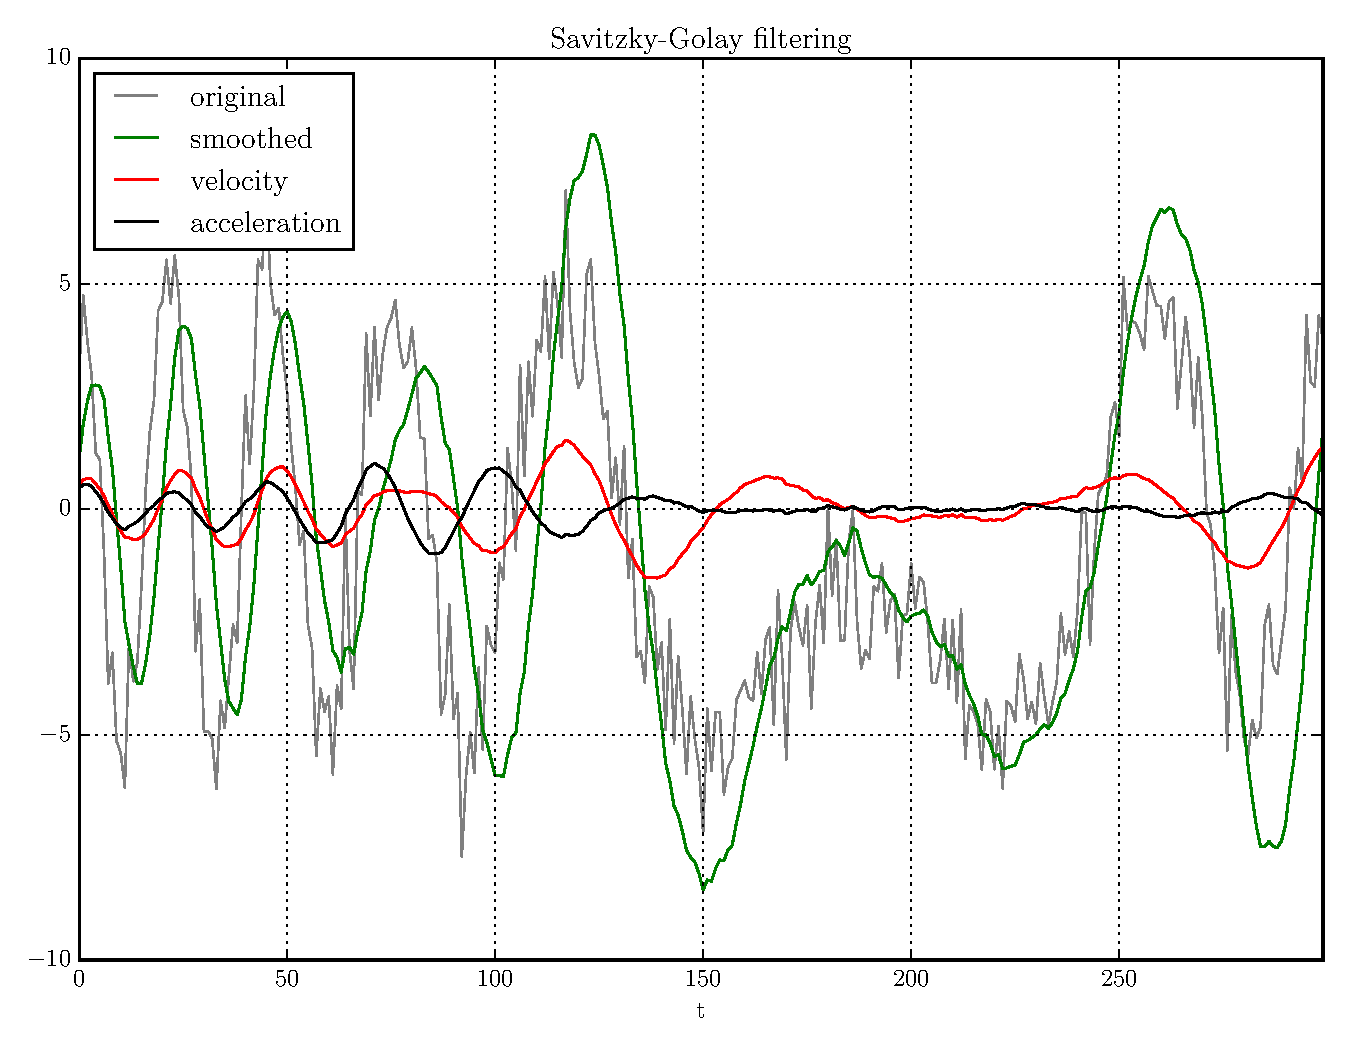
\includegraphics[scale=0.30]{../img/savgol.pdf}
\caption{Savitzky-Golay filtering of a signal with added Gaussian noise. The smoothing window is 50 points, centered at the far right.} 
\label{fig:savgol}
\end{figure}
\end{frame}

\subsubsection*{Matching in Graphs}
\begin{frame} \frametitle{Maximum Weight Matching}
\begin{figure}
\centering
\includegraphics[scale=0.5]{../img/matching.tex}
\end{figure}
Let $G=(V,E)$ a graph:
\begin{itemize}
\item \emph{maximum weight matching} $M\subseteq E$ : a subset of edges where 
\begin{itemize}
\item no two edges share a common vertex
\item largest possible number of edges
\item maximizes the sum of weights
\end{itemize}
\end{itemize}
\end{frame}

\begin{frame} \frametitle{Maximum Weight Matching}\framesubtitle{The Primal-Dual Method}
\setbeamercolor{block title}{use=structure,fg=black,bg=blue!5!white}
\setbeamercolor{block body}{use=structure,fg=black,bg=blue!5!white}

\begin{block}{}
\vspace{-0.4cm}
\begin{align*}
\begin{split}
\text{Constraints in Primal}&\Longleftrightarrow \text{Variables in Dual}\\
\text{Constraints in Dual}\quad &\Longleftrightarrow \text{Variables in Primal}
\end{split}
\end{align*}
\end{block}
\vspace{0.4cm}
\begin{columns}
\begin{column}[t]{0.49\textwidth}
\vspace{-1.5cm}
\begin{align*}
\intertext{\textbf{The primal}:}
\max&\quad \sum_{(u,v) \in E} x_{u,v} w_{u,v}\\
\text{s.t.} &\qquad x_{u,v}\geq 0 &&, (u,v) \in E \\
	&\quad \sum_{u \in e: e\in E} x_e \leq 1 &&, u \in V
\end{align*}\end{column}
\begin{column}[t]{0.49\textwidth}
\vspace{-1.5cm}
\begin{align*}
\intertext{\textbf{The dual}:}
\min&\quad \sum_{u \in V} y_u\\
\text{s.t.} &\quad y_u\geq 0 &&, u \in V\\
	&\quad y_u+y_v \geq w_{u,v} &&,(u,v) \in E
\end{align*}
\end{column}
\end{columns}
\end{frame}

%%%%%%%%%%%%%  section: IMPL  %%%%%%%%%%%%%%%%%%%%%%%
\section{Problem Statement \& Implementation}
\begin{frame}
  \tableofcontents[currentsection]
\end{frame}
 
\subsection{Problem Statement}
\begin{frame} \frametitle{Problem Formulation}
\textbf{Reduce the communication burden} of the \emph{Geometric Monitoring} method by:
\begin{itemize}
\item Optimally position \emph{drift vectors} during the \emph{balancing process}
\item Appropriate node selection for inclusion in the \emph{balancing set}
\end{itemize}
,in order to \textbf{increase scalability} in terms of:
\begin{itemize}
\item node popullation
\item stream dimensionality.
\end{itemize}
\end{frame}
\subsection{Implementation}

\begin{frame} \frametitle{The Geometric Monitoring Framework} \framesubtitle{Assumptions}
\begin{itemize}
\item Coordinator-based scenario
\item Instantaneous, loss-less, reliable communication
\item Iterative operation based on time-steps
\item System pause during violation resolution
\item Coordinator node does not monitor a stream
\end{itemize}
\end{frame}

\subsubsection*{Distance-based Hierarchical Clustering}
\begin{frame} \frametitle{The Distance-based Hierarchical Clustering}\framesubtitle{The Idea}
Node selection for \emph{violation resolution}:
\begin{itemize}
\item Elevate \emph{randomness} of the initial \emph{geometric monitoring} method {\tiny(\fullcite{Sharfman2006GM})}
\item Hierarchical node clustering scheme {\tiny(\fullcite{Keren2014GMHetStreams})}
\item Decouple matching from the data distribution at the nodes {\tiny(\fullcite{Keren2014GMHetStreams})}
\item Accurately follow \emph{global statistics vector}
\item Node ``cancel each other out'' during the \emph{balancing process}
\end{itemize}
\end{frame}

\begin{frame} \frametitle{The Distance-based Hierarchical Clustering}\framesubtitle{The Weight Function}
\setbeamercolor{block title}{use=structure,fg=white,bg=blue!55!black}
\setbeamercolor{block body}{use=structure,fg=black,bg=blue!5!white}
\begin{block}{Weight function}
\vspace{0.2cm}
\begin{equation*}
w_{i,j}=
\sum_{t=t_0}^{t_{end}}{[(f(\vec{v}_{global}(t))-f(\frac{\vec{v_i}(t)+\vec{v_j}(t)}{2}))+(|\vec{v_i}(t)-\vec{v_j}(t)|)]}
\end{equation*}
\vspace{0.2cm}
\end{block}
\end{frame}

\begin{frame} \frametitle{The Distance-based Hierarchical Clustering}\framesubtitle{Example}
\begin{figure}
\begin{columns}
\begin{column}[t]{0.4\linewidth}
\vspace{-5.5cm}\caption{Distance based node matching operating on 4 nodes ($\{n_0, n_1, n_2, n_3\}$). Distance $d_1$ : the distance of the data vector mean of the paired nodes $n_0$ and $n_3$ from the global mean (\emph{global data vector}), distance $d_2$ : denotes the in-between distance of data vectors $\vec{v_0}(t)$ and $\vec{v_3}(t)$ of the node pair. Both distances are taking part in the edge weighting process.}
\end{column}
\begin{column}[t]{0.6\linewidth}
\centering
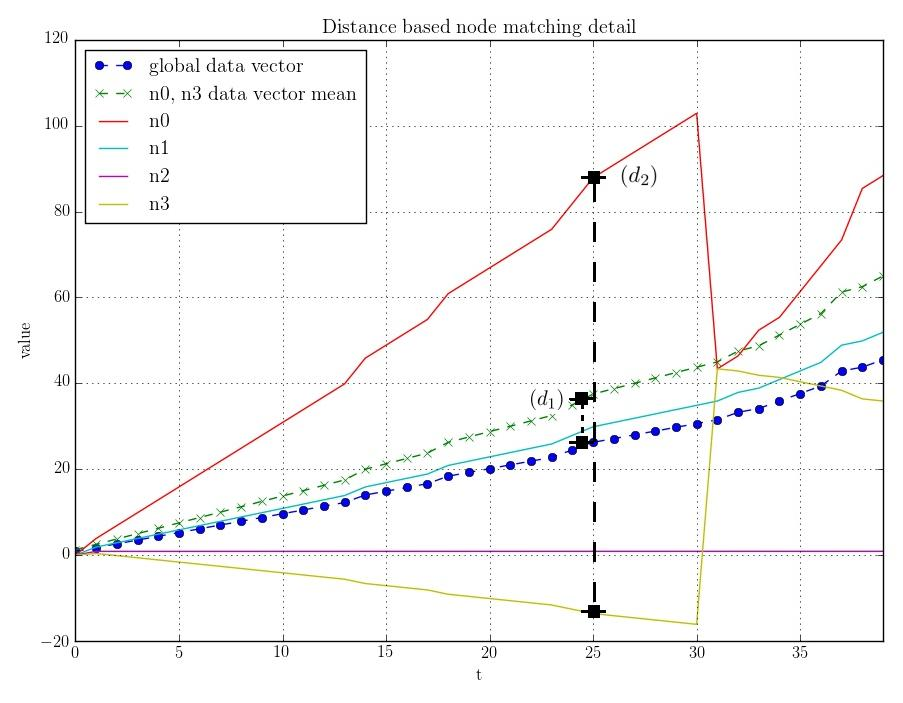
\includegraphics[scale=0.22]{../img/distoptpair_example_detail_edited.jpeg}
\end{column}
\end{columns}
\end{figure}
\end{frame}

\subsubsection*{Heuristic Balancing}
\begin{frame} \frametitle{The Heuristic Balancing}\framesubtitle{The Idea}
In prior work:
\begin{itemize}
\item identical handling of nodes during the balancing process
\item ignore stream idiosyncrasies and monitoring function peculiarities
\end{itemize}
The \emph{heuristic balancing} method:
\begin{itemize}
\item optimally position \emph{drift vectors in space}
\item take into account stream behaviour (\emph{velocity} and \emph{acceleration})
\end{itemize}
\end{frame}

\begin{frame} \frametitle{The Heuristic Balancing}\framesubtitle{The Optimizing Function}
\setbeamercolor{block title}{use=structure,fg=white,bg=blue!55!black}
\setbeamercolor{block body}{use=structure,fg=black,bg=blue!5!white}
\begin{block}{Weight function}
\vspace{0.2cm}
\begin{equation*}
\max\min \frac{(T-x_i)-accel_i(t_{lv})*t^2}{vel_i(t_{lv})}, \forall n_i \in P'
\end{equation*}
\end{block}
where:
\scalebox{0.7}{
\begin{minipage}[t]{\linewidth}
\vspace{-0.5cm}
\begin{align*}
t&:\text{the variable to optimize}\\
T&:\text{monitoring threshold}\\
x_i&:\text{the maximum value of the monitoring function $f(\cdot)$ over the bounding ball $B(\vec{e}(t_{lv}), \vec{u_i}(t_{lv}))$,}\\
vel_i(t_{lv})&:\text{the estimated velocity of the maximum value of the monitoring function $f(\cdot)$}\\
accel_i(t_{lv})&:\text{the estimated acceleration of the maximum value of the monitoring function $f(\cdot)$}\\
t_{lv}&:\text{time of Local Violation occurrence}\\
P'&:\text{the balancing set}
\end{align*}
\end{minipage}
}
\end{frame}

\begin{frame}\frametitle{The Heuristic Balancing}\framesubtitle{Example}
\begin{columns}
\begin{column}[t]{0.5\linewidth}
\begin{figure}
\vspace{-1.2cm}
\includegraphics[scale=0.32]{../img/classic_balancing.tex}
\caption{The classic balancing method.} 
\end{figure}
\end{column}
\begin{column}[t]{0.5\linewidth}
\begin{figure}
\vspace{-1.2cm}
\includegraphics[scale=0.32]{../img/heuristic_balancing.tex}
\caption{The heuristic balancing method.} 
\end{figure}
\end{column}
\end{columns}
\end{frame}

%%%%%%%%%%%%%  section: EXPERIMENTS  %%%%%%%%%%%%%%%%%%%%%%%
\section{Experimental Results}
\begin{frame}
  \tableofcontents[currentsection]
\end{frame}

\subsection{Data \& Setup}
\begin{frame}\frametitle{Acronyms for Implemented Methods}
\begin{itemize}
\item[] GM: the initial geometric monitoring method {\tiny(\fullcite{Sharfman2006GM})}
\item[] HM: the proposed heuristic balancing process
\item[] DIST: the proposed distance-based hierarchical node clustering
\item[] DISTR: the distribution-based hierarchical node clustering {\tiny(\fullcite{Keren2014GMHetStreams})}
\end{itemize}
\end{frame}

\subsubsection*{Synthetic Data}
\begin{frame} \frametitle{Synthetic Data}
\begin{itemize}
\item $v_i(t_{k+1})=v_i(t_k) + (1-\lambda)u_{k} + \lambda u_{k+1}$
\item 1-dimensional
\item Velocities sampled from user-specified Gaussian distribution
\item $\lambda$ smoothing parameter
\item Additive Gaussian noise
\item 3 sets of datasets: \emph{LIN}, \emph{INT}, \emph{NOISE}
\item First 20\% of data streams used as training data, when needed
\end{itemize}
\end{frame}

\begin{frame}\frametitle{Synthetic Data}\framesubtitle{Examples}
\begin{columns}
\begin{column}[t]{0.32\linewidth}
\begin{figure}
\vspace{-1cm}
\centering
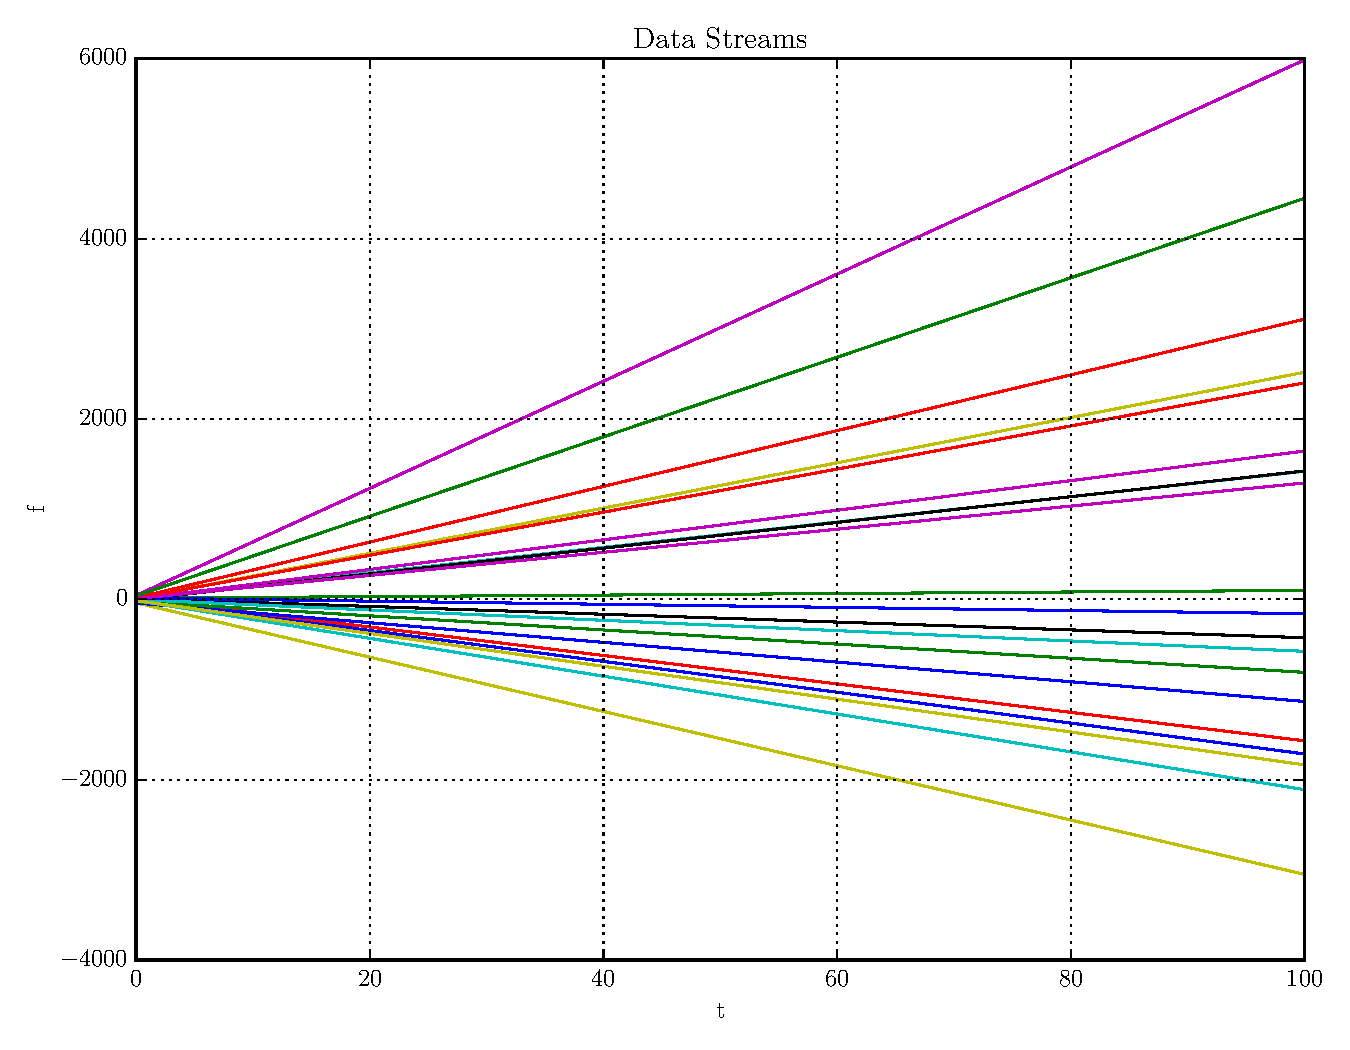
\includegraphics[scale=0.16]{../img/linear1D20N_streams.pdf}
\caption{\emph{LIN} local statistics streams of 20 nodes} 
\end{figure}
\end{column}
\begin{column}[t]{0.32\linewidth}
\begin{figure}
\vspace{-1cm}
\centering
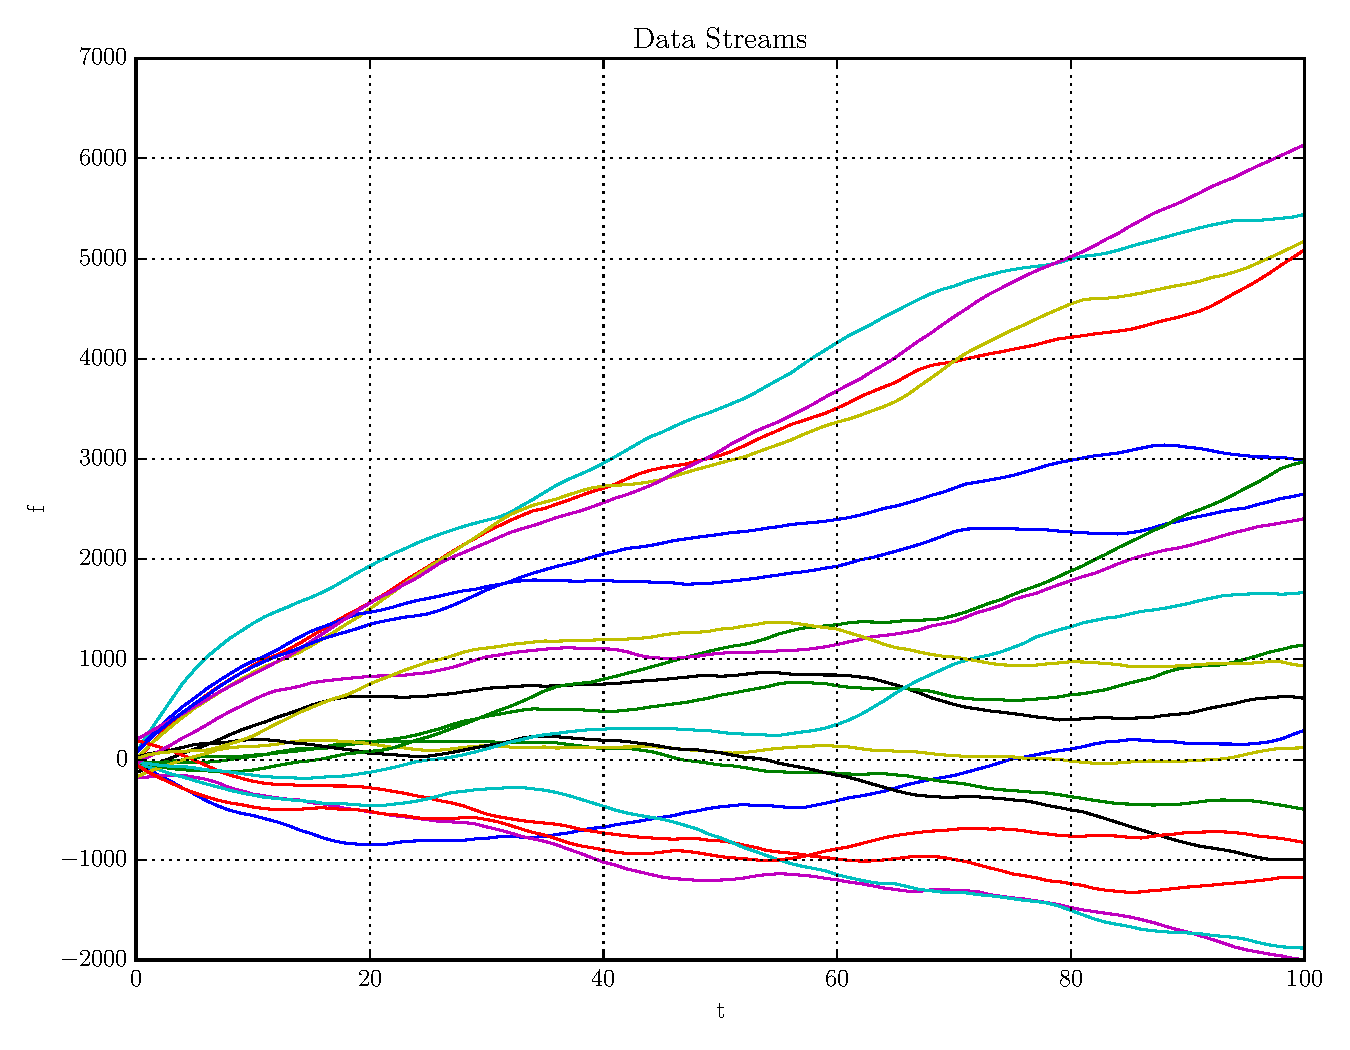
\includegraphics[scale=0.16]{../img/interweaving1D20N_streams.pdf}
\caption{\emph{INT} local statistics streams of 20 nodes} 
\end{figure}
\end{column}
\begin{column}[t]{0.32\linewidth}
\begin{figure}
\vspace{-1cm}
\centering
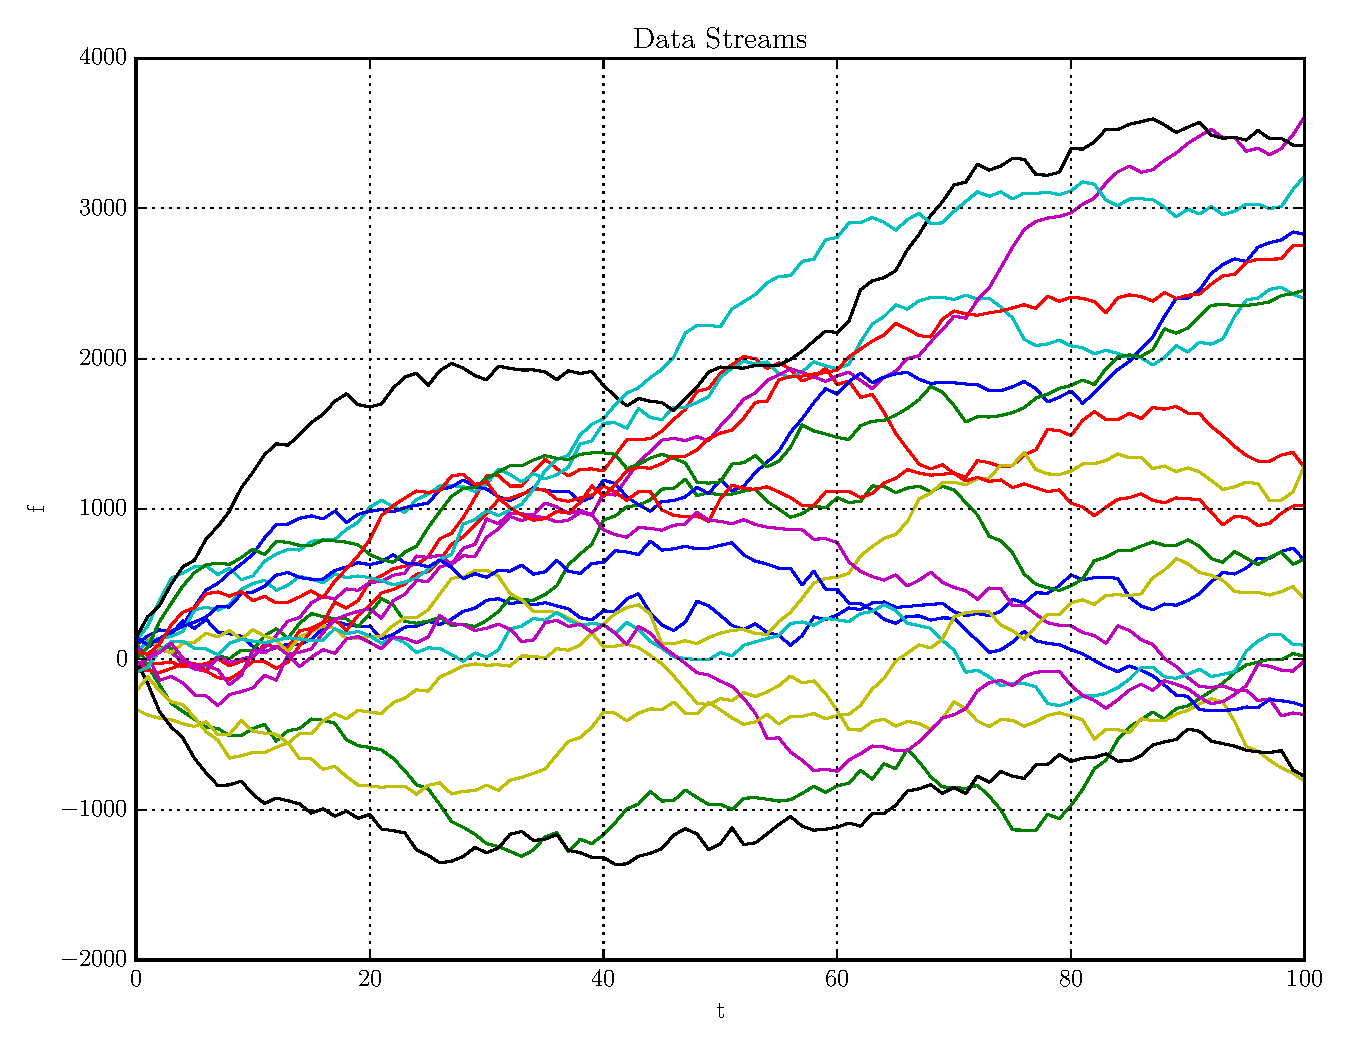
\includegraphics[scale=0.16]{../img/noisyinterweaving1D20N_streams.pdf}
\caption{\emph{NOISE} local statistics streams of 20 nodes} 
\end{figure}
\end{column}
\end{columns}
\end{frame}

\subsubsection*{Real-world Data}
\begin{frame} \frametitle{Real-world Data}
\begin{itemize}
\item ``European Environmental Agency - AQ e-Reporting'' database {\tiny(\fullcite{AirBase})}
\item Hourly measurements of $NO_2$ and $NO$, in micro-grams per cubic meter, averaged over a window of five days for a whole year.
\item Nodes correspond to randomly selected air quality measurement stations across Austria.
\item First month of measurements used as training data, when needed.
\end{itemize}
\end{frame}

\subsubsection*{Real-world Data}
\begin{frame} \frametitle{Real-world Data}\framesubtitle{Examples}
\begin{columns}
\begin{column}[t]{0.5\linewidth}
\begin{figure}
\centering
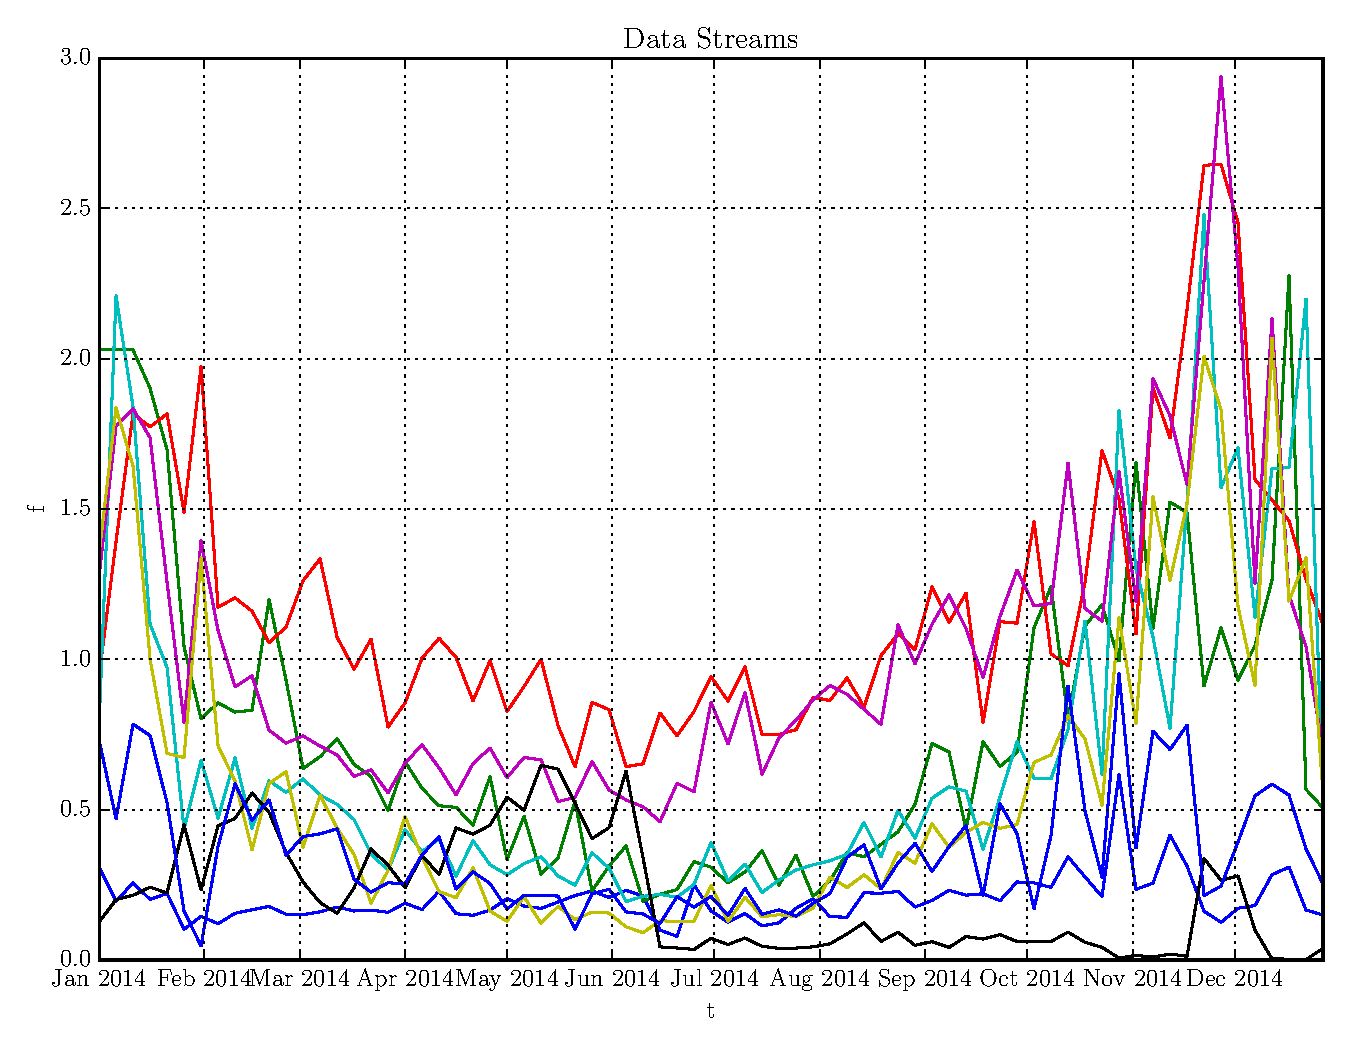
\includegraphics[scale=0.2]{../img/AT_NO2_NO_2014_8N_streams.pdf}
\caption{Streams of 8 nodes monitoring the ratio $NO/NO_2$.} 
\end{figure}
\end{column}
\begin{column}[t]{0.5\linewidth}
\begin{figure}
\centering
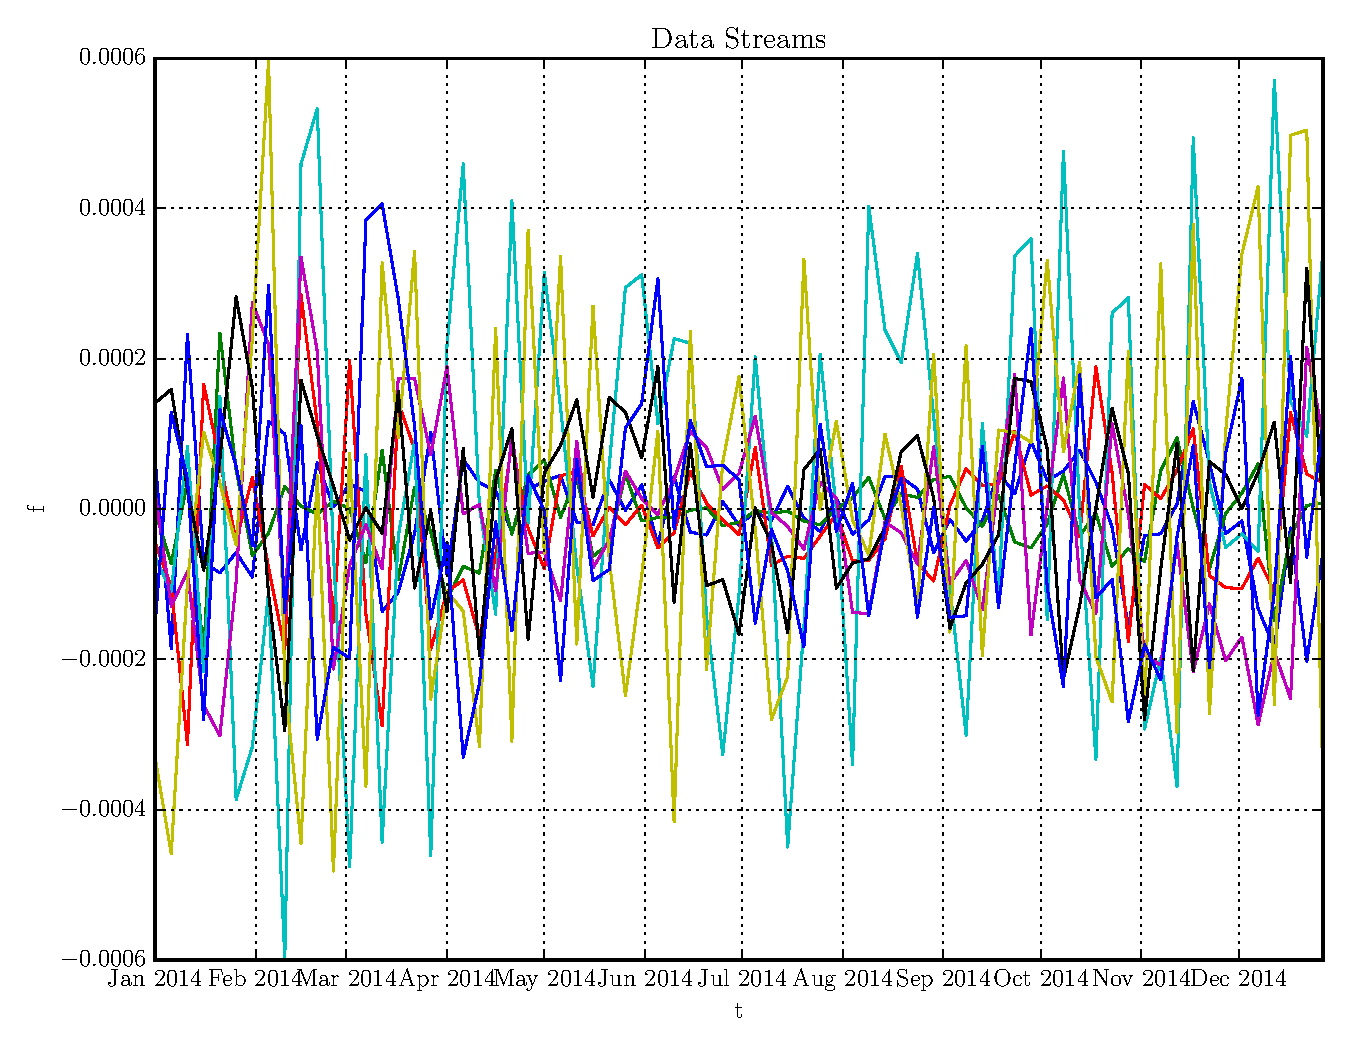
\includegraphics[scale=0.2]{../img/AT_NO2_sq_2014_8N_streams.pdf}
\caption{Streams of 8 nodes monitoring the variance of $NO_2$ air pollutant.} 
\end{figure}
\end{column}
\end{columns}
\end{frame}

\subsection{Experiments}

\subsubsection*{ Matching Algorithms}
\begin{frame} \frametitle{GM, DIST, DISTR Comparison} \framesubtitle{\emph{LIN} dataset}
\begin{figure}
\vspace{-0.5cm}
\centering
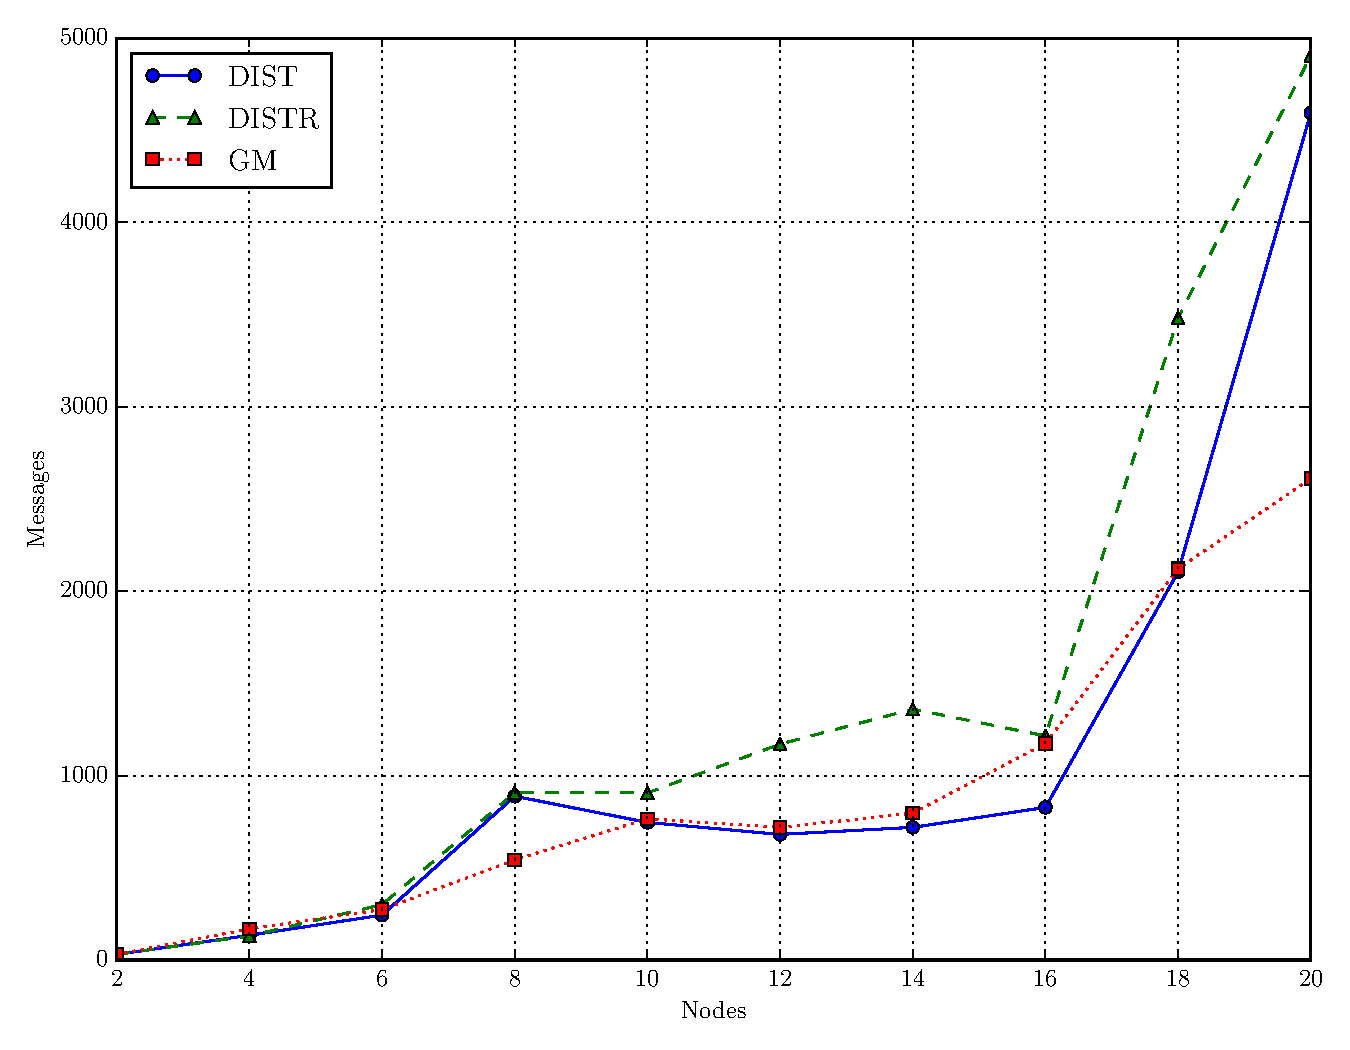
\includegraphics[scale=0.3]{../img/matching_msg_linear.pdf}
  \caption{Communication costs of methods GM, DISTR and DIST for the \emph{LIN} dataset.}
\end{figure}
\end{frame}

\begin{frame} \frametitle{GM, DIST, DISTR Comparison}\framesubtitle{\emph{INT} dataset}
\begin{figure}
\vspace{-0.5cm}
\centering
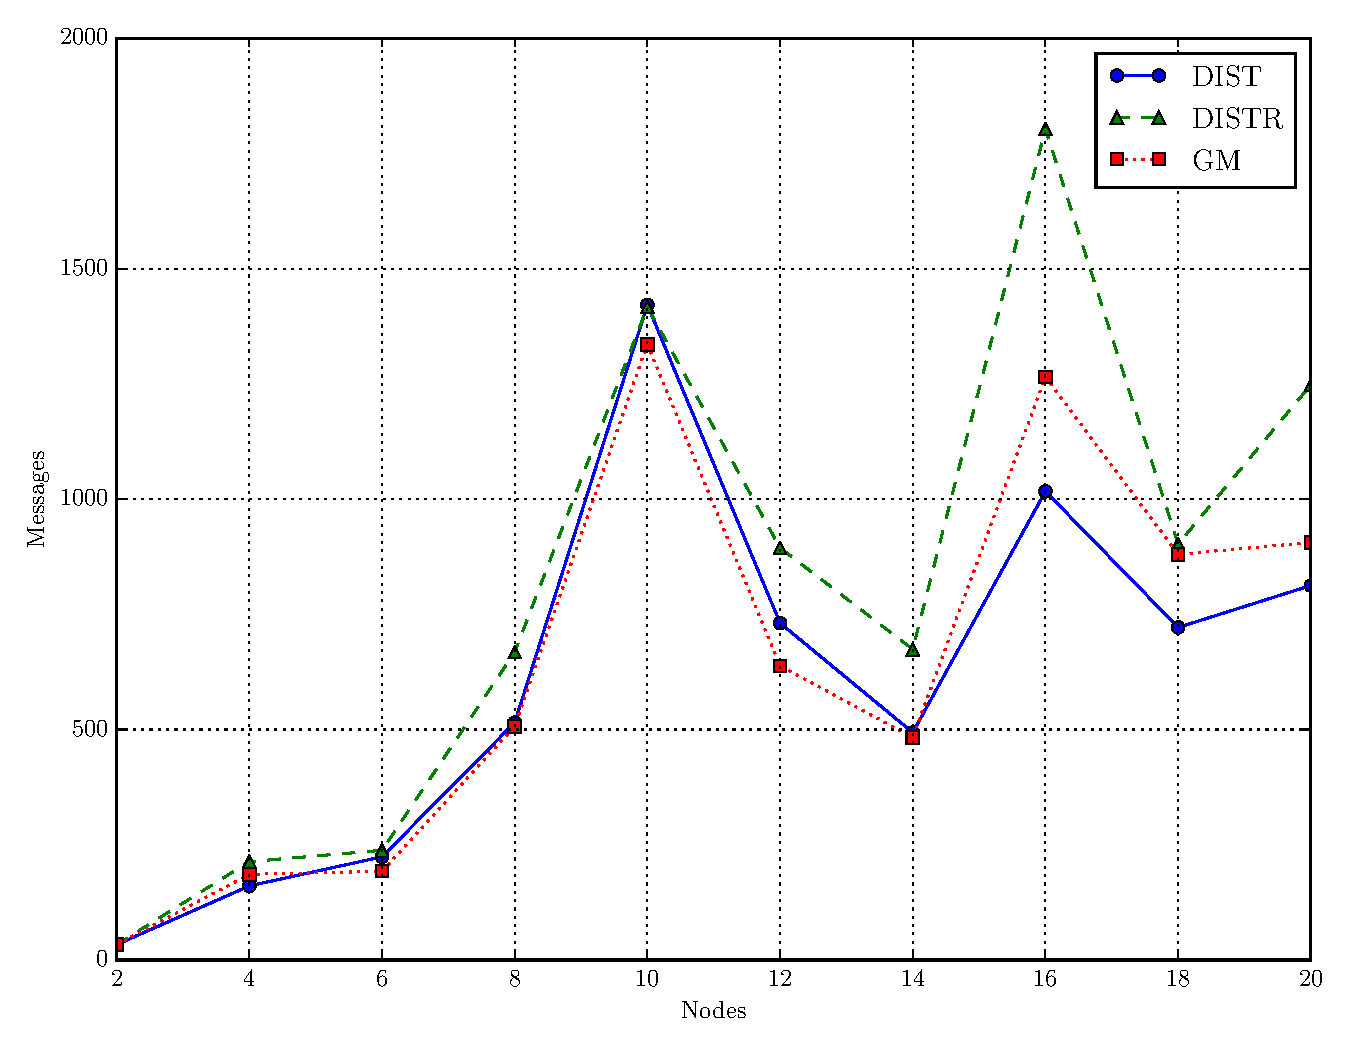
\includegraphics[scale=0.3]{../img/matching_msg_interweaving.pdf}
  \caption{Communication costs of methods GM, DISTR and DIST for the \emph{INT} dataset.}
\end{figure}
\end{frame}

\begin{frame} \frametitle{GM, DIST, DISTR Comparison}\framesubtitle{\emph{NOISE} dataset}
\begin{figure}
\vspace{-0.5cm}
\centering
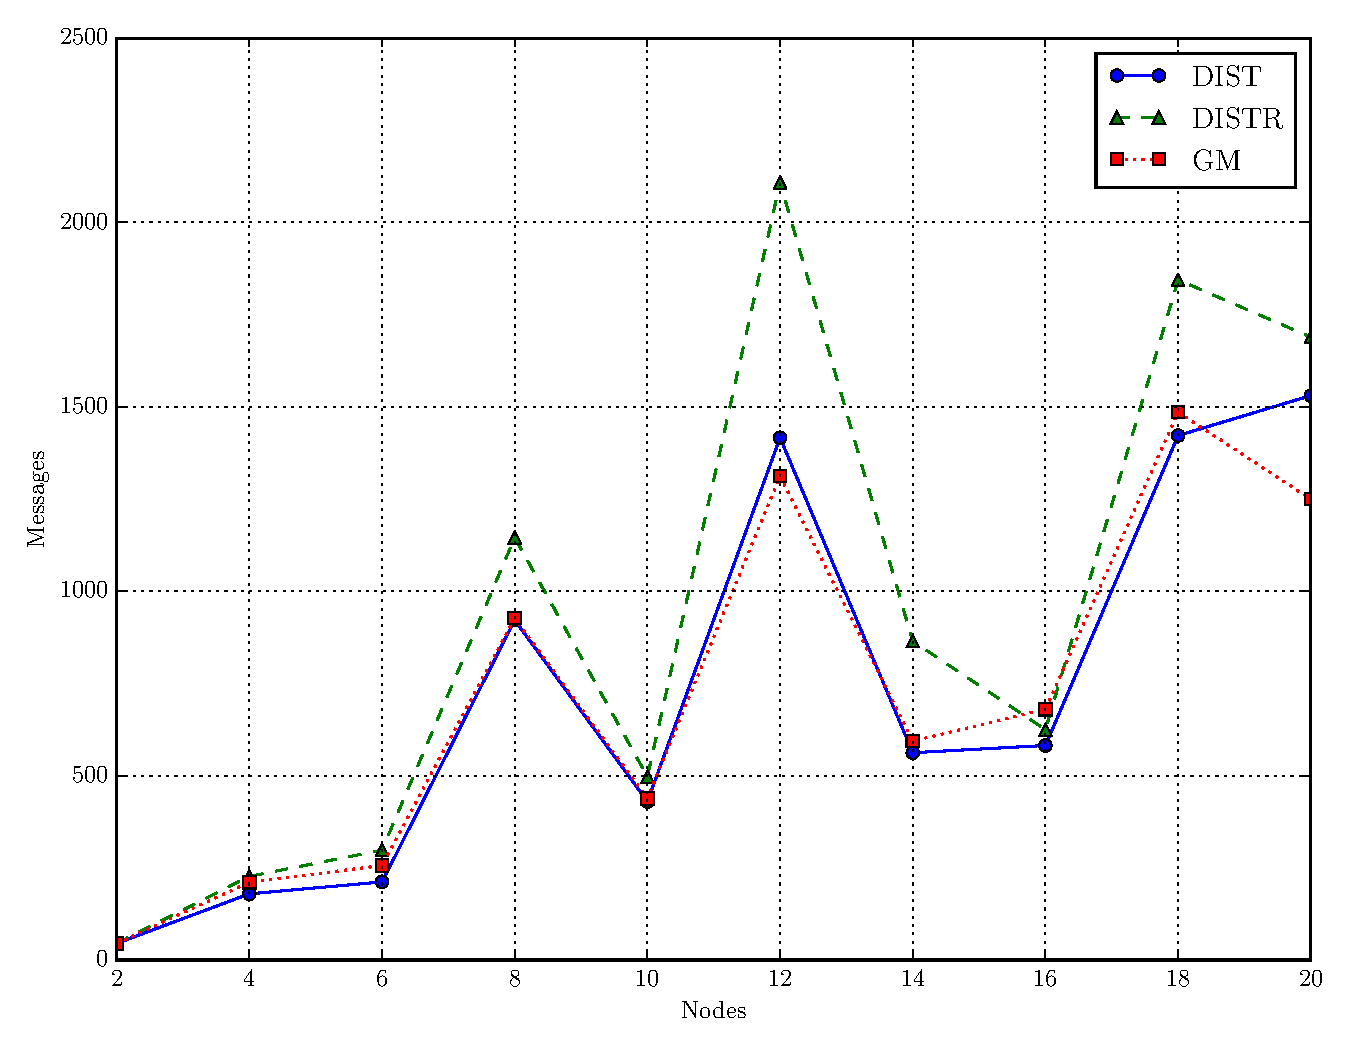
\includegraphics[scale=0.3]{../img/matching_msg_noisyinterweaving.pdf}
  \caption{Communication costs of methods GM, DISTR and DIST for the \emph{NOISE} dataset.}
\end{figure}
\end{frame}

\begin{frame} \frametitle{GM, DIST, DISTR Comparison} \framesubtitle{\emph{LIN} dataset}
\begin{figure}
\vspace{-0.2cm}
\centering
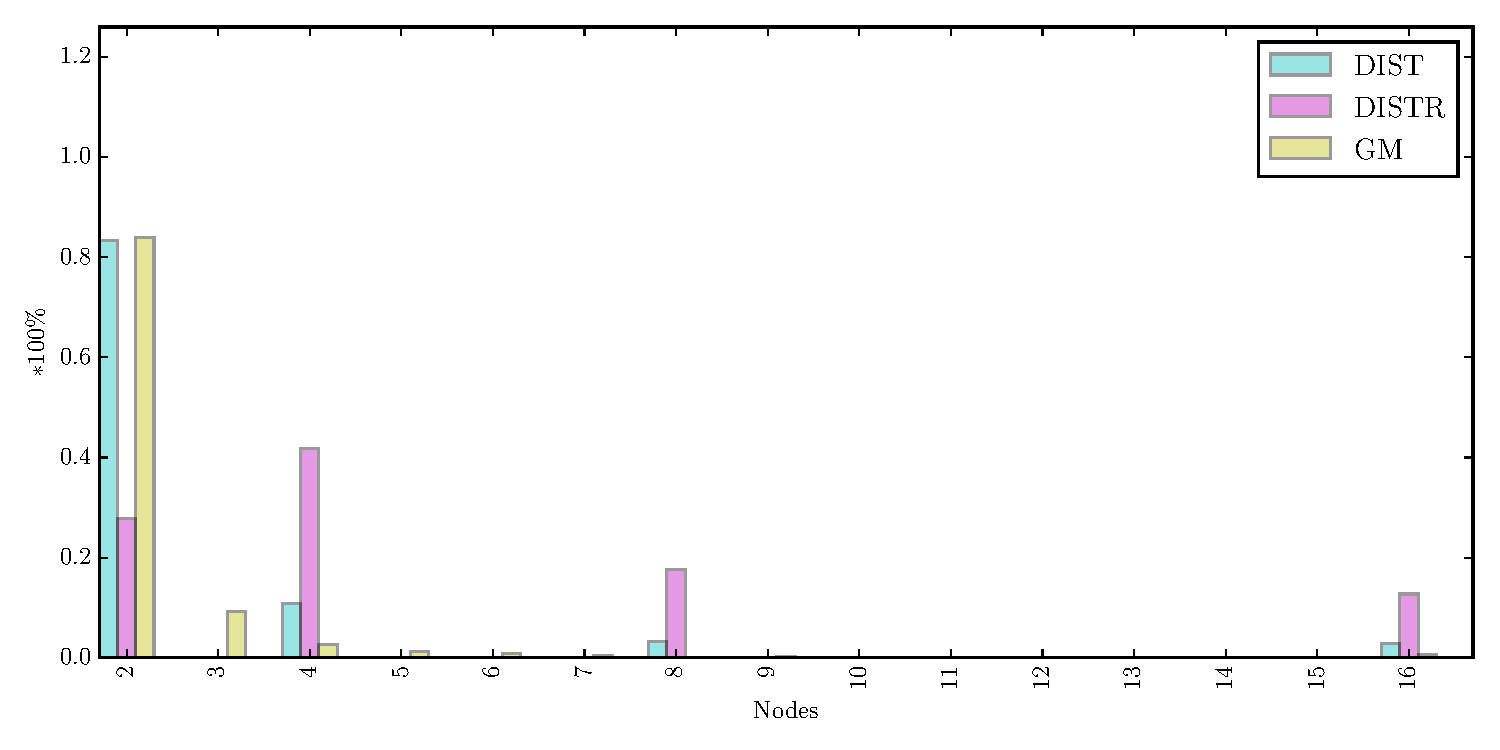
\includegraphics[scale=0.4]{../img/matchings_matchings_linear.pdf}
  \caption{Number of nodes participating in violation resolutions as a fraction of total Local Violations, for the \emph{LIN} dataset.}
\end{figure}
\end{frame}

\begin{frame} \frametitle{GM, DIST, DISTR Comparison}\framesubtitle{\emph{INT} dataset}
\begin{figure}
\vspace{-0.2cm}
\centering
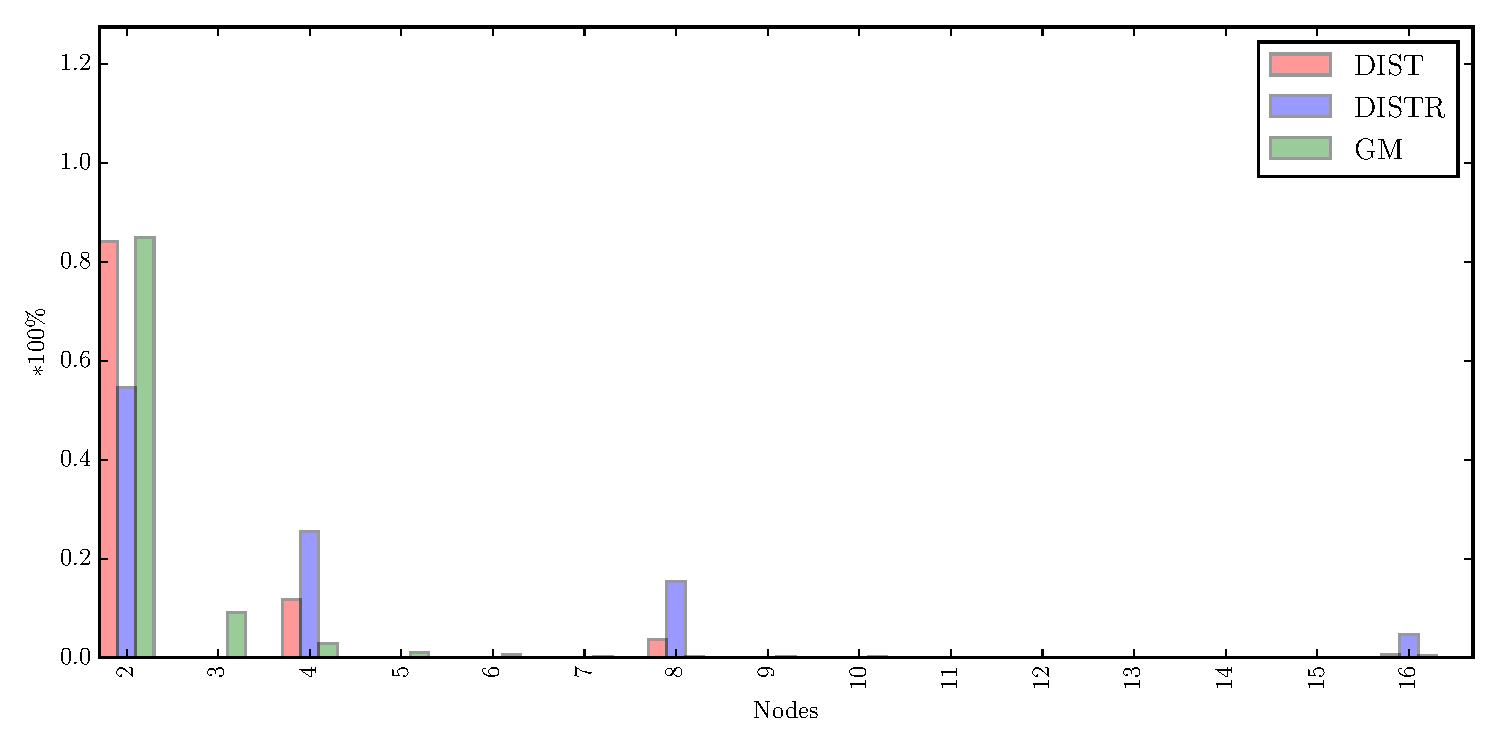
\includegraphics[scale=0.4]{../img/matchings_matchings_interweaving.pdf}
  \caption{Number of nodes participating in violation resolutions as a fraction of total Local Violations, for the \emph{INT} dataset.}
\end{figure}
\end{frame}

\begin{frame} \frametitle{GM, DIST, DISTR Comparison}\framesubtitle{\emph{NOISE} dataset}
\begin{figure}
\vspace{-0.2cm}
\centering
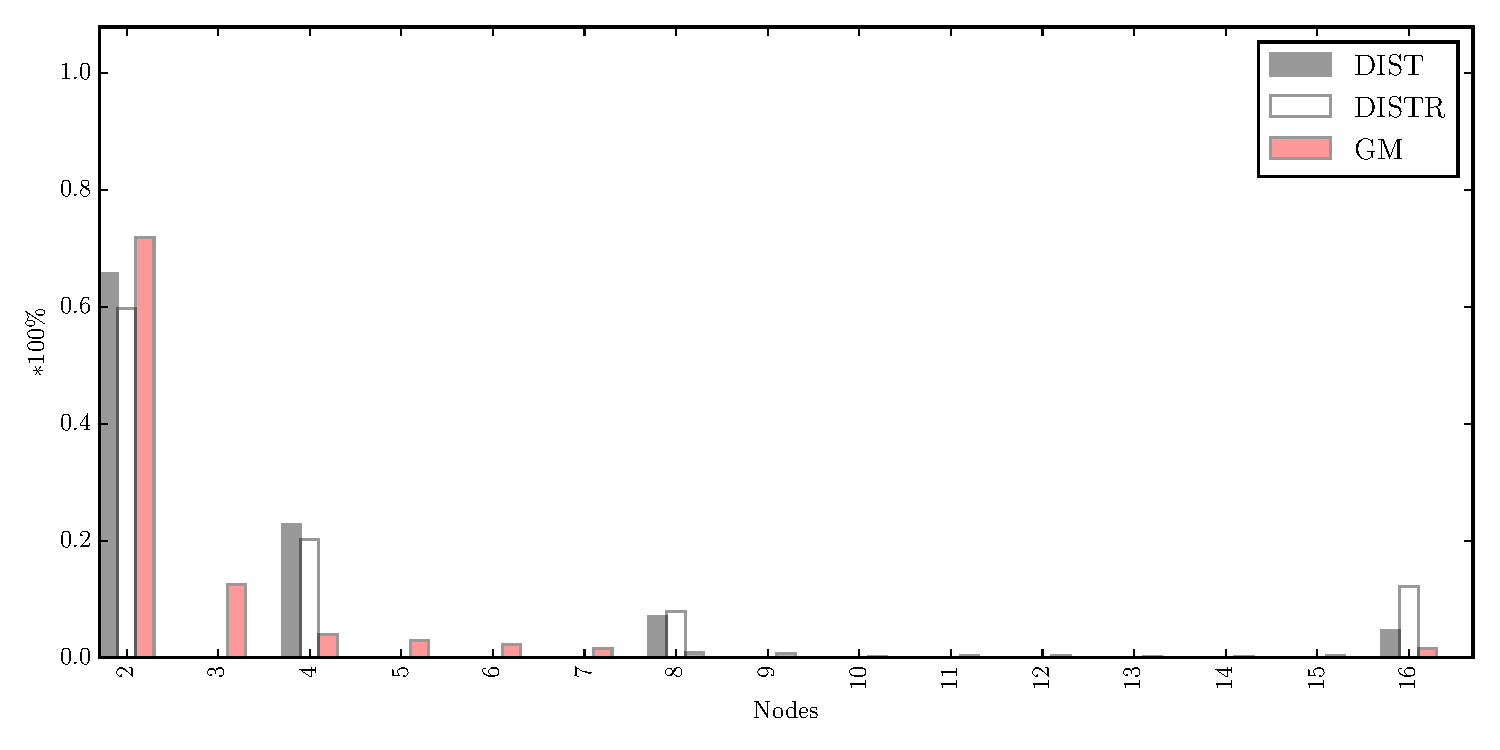
\includegraphics[scale=0.4]{../img/matchings_matchings_noisyinterweaving.pdf}
  \caption{Number of nodes participating in violation resolutions as a fraction of total Local Violations, for the \emph{NOISE} dataset.}
\end{figure}
\end{frame}

\subsubsection*{Balancing Methods}
\begin{frame} \frametitle{GM, HM Comparison} \framesubtitle{Messages}
\begin{columns}
\begin{column}[t]{0.5\linewidth}
\begin{figure}
\vspace{-1cm}
\centering
  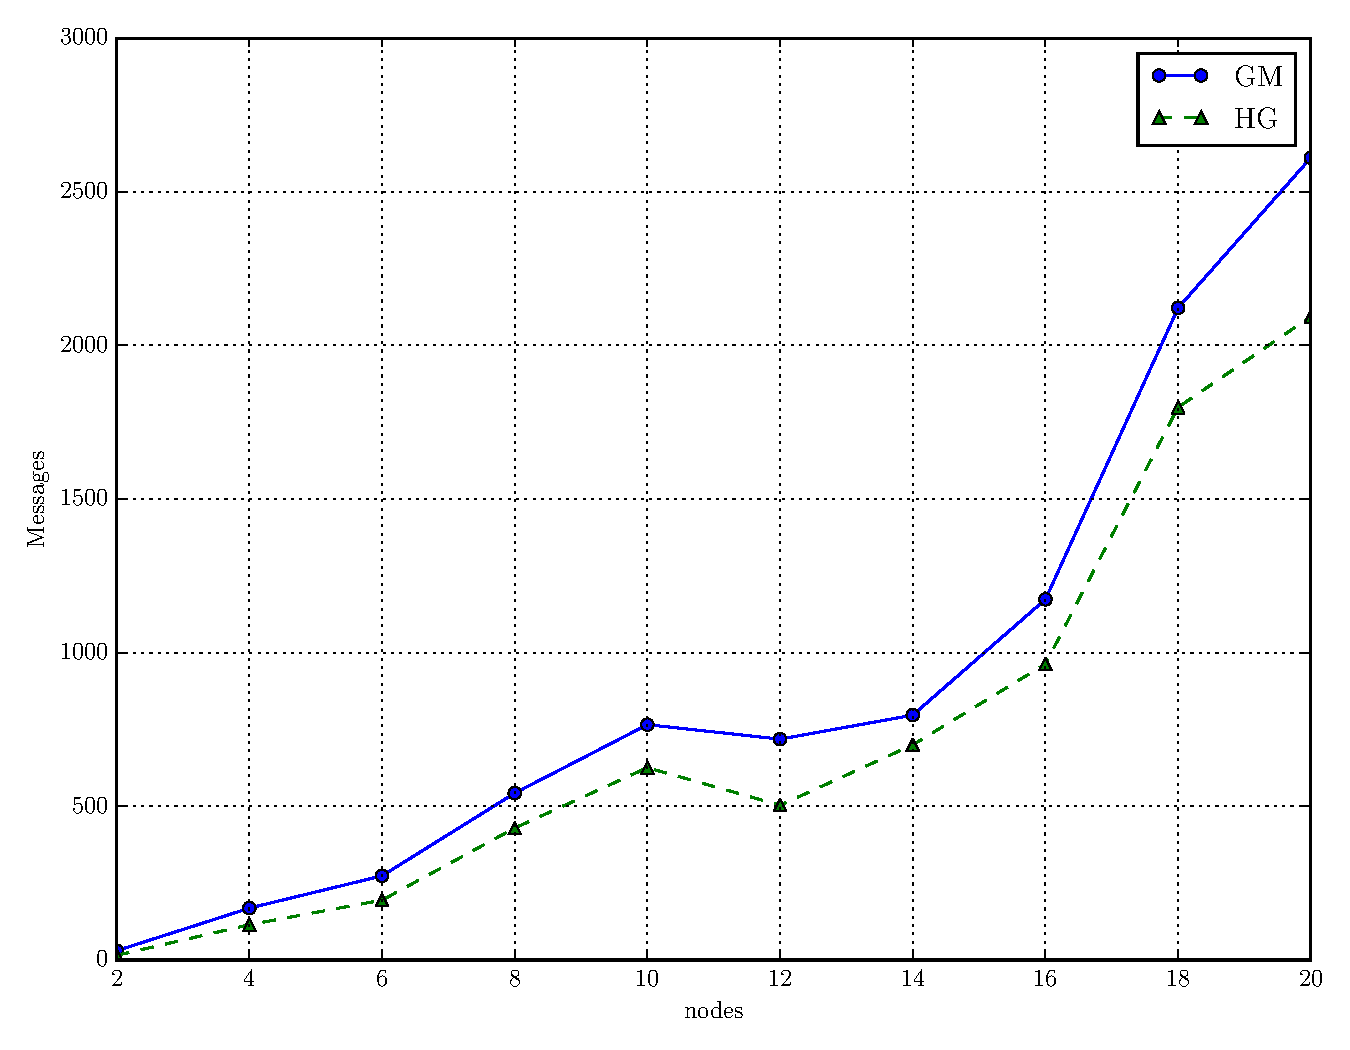
\includegraphics[scale=0.25]{../img/bal_msg_linear_nodes.pdf}
  \caption{Communication cost of methods GM and HM for the \emph{LIN} dataset.}
\end{figure}
\end{column}
\begin{column}[t]{0.5\linewidth}
\begin{figure}
\vspace{-1cm}
\centering
  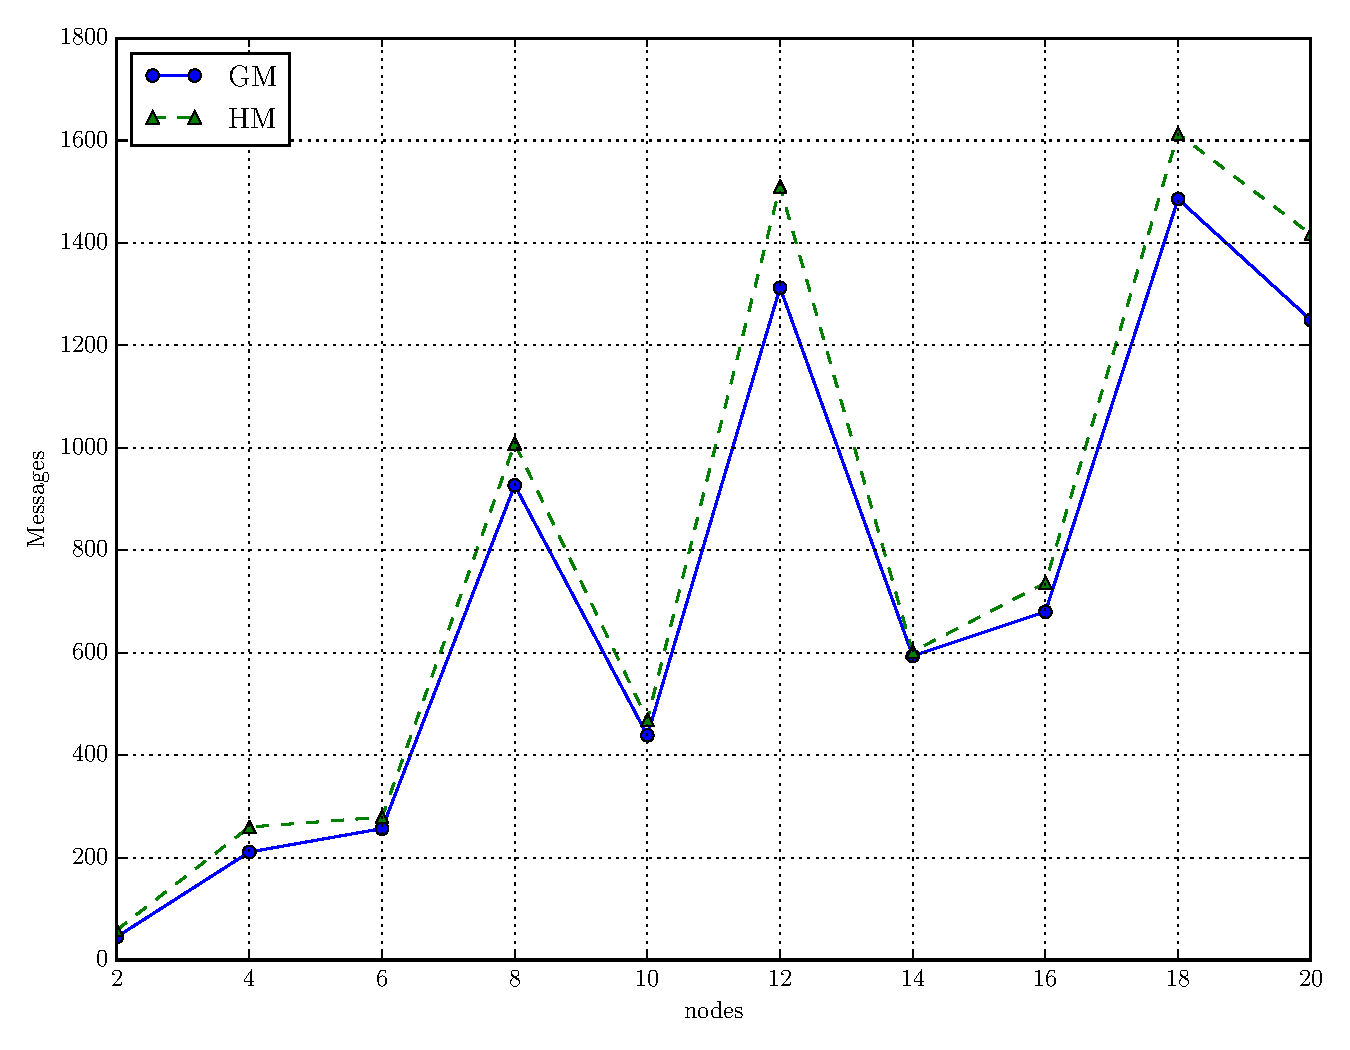
\includegraphics[scale=0.25]{../img/bal_msg_noisyinterweaving_nodes.pdf}
  \caption{Communication cost of methods GM and HM for the \emph{NOISE} dataset.}
\end{figure}
\end{column}
\end{columns}
\end{frame}

\begin{frame} \frametitle{GM, HM Comparison} \framesubtitle{Drift vectors}
\begin{columns}
\begin{column}[t]{0.5\linewidth}
\begin{figure}
\vspace{-1cm}
\centering
  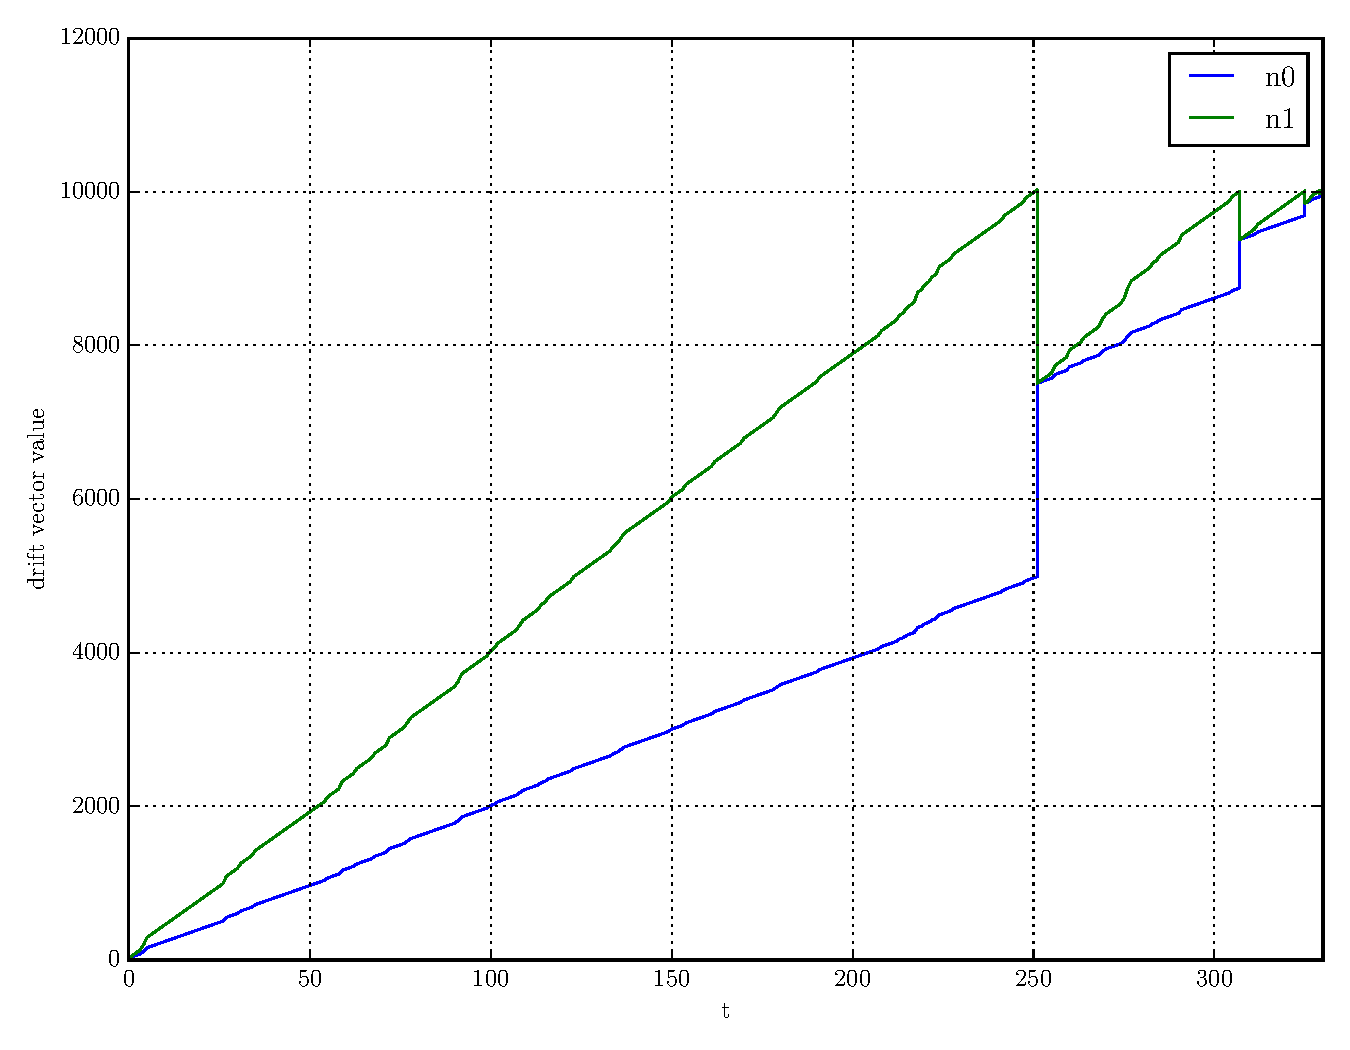
\includegraphics[scale=0.25]{../img/bal_classic_drifts_linear2N.pdf}
  \caption{Drift vectors of 2 nodes, as formulated by the GM algorithm.}
\end{figure}
\end{column}
\begin{column}[t]{0.5\linewidth}
\begin{figure}
\vspace{-1cm}
\centering
  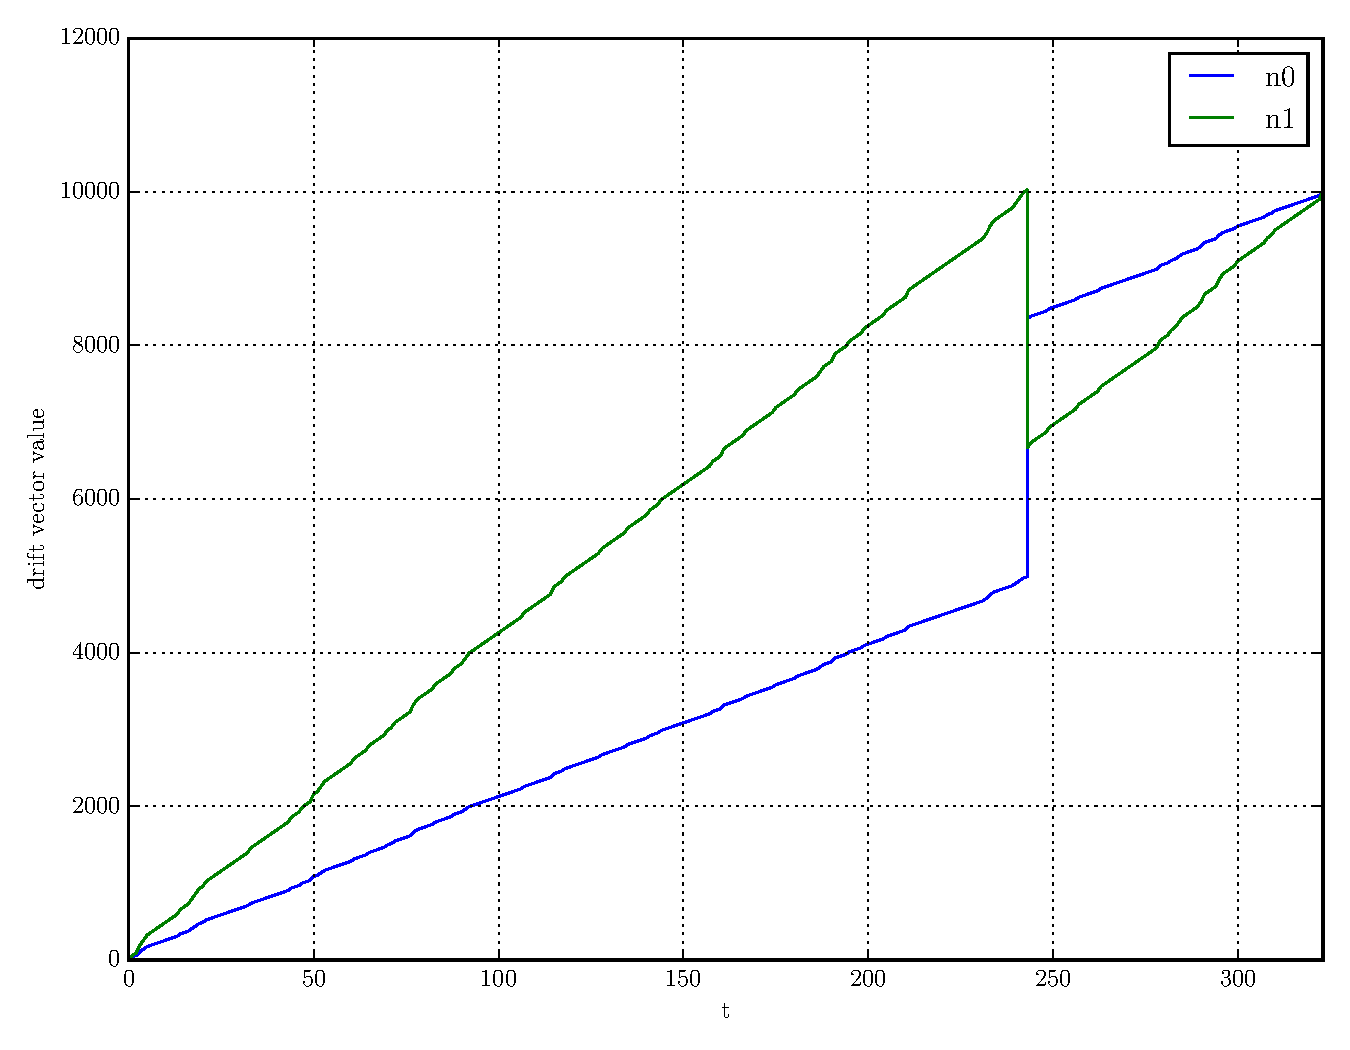
\includegraphics[scale=0.25]{../img/bal_heuristic_drifts_linear2N.pdf}
  \caption{Drift vectors of 2 nodes, as formulated by the HM algorithm.}
\end{figure}
\end{column}
\end{columns}
\end{frame}

\subsubsection*{Synthetic Data}
\begin{frame} \frametitle{GM, HDM Comparison}\framesubtitle{\emph{LIN}}
\begin{figure}
\vspace{-0.5cm}
\centering
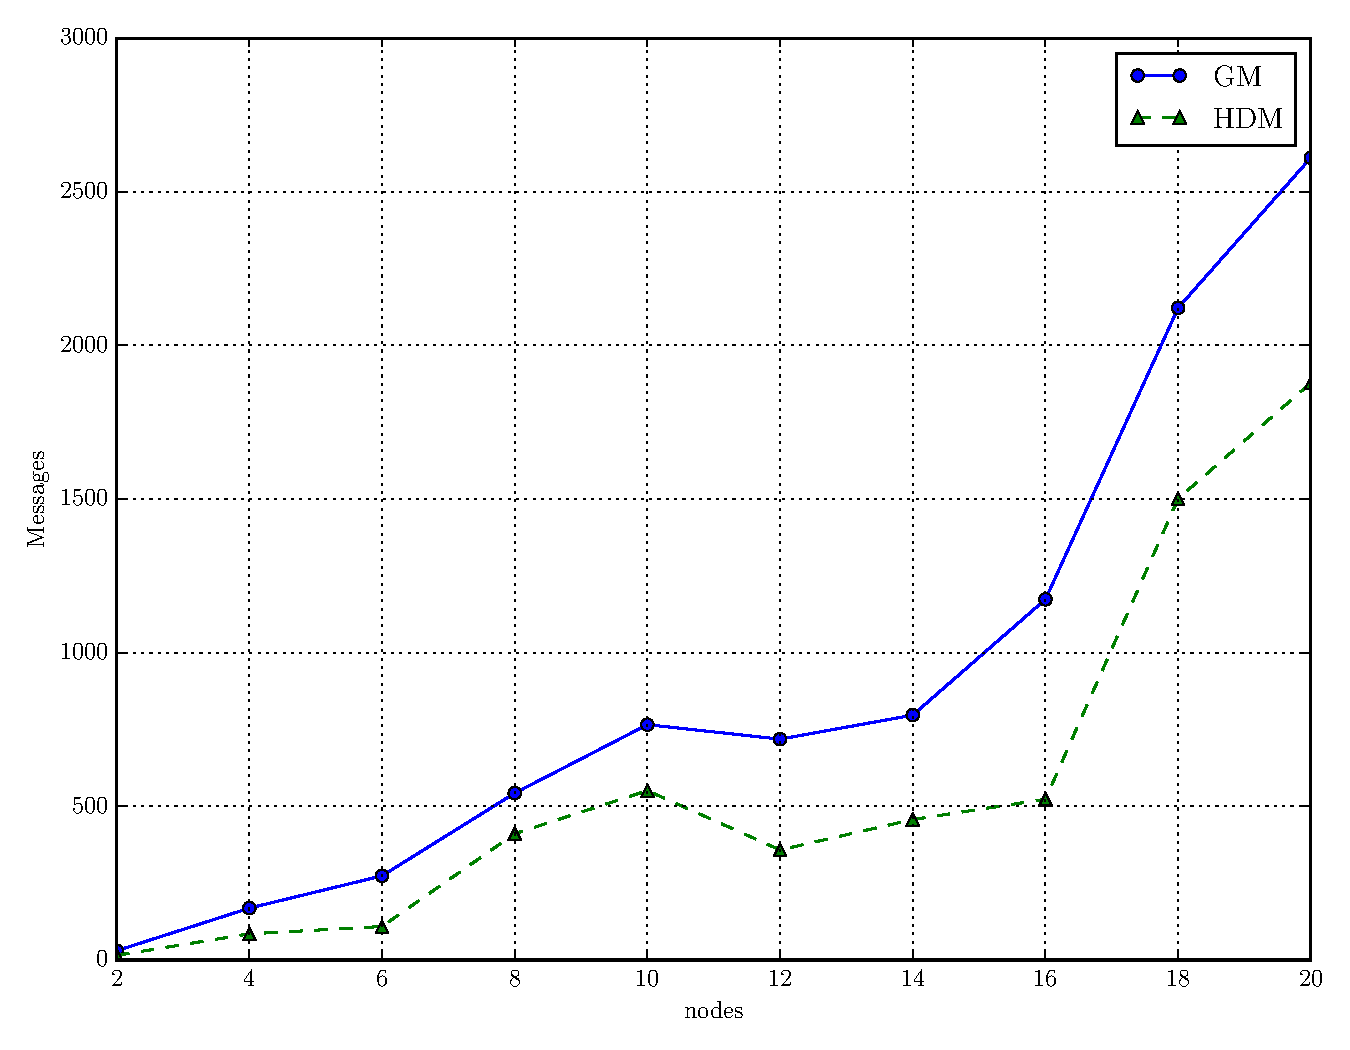
\includegraphics[scale=0.3]{../img/main_msg_linear_nodes.pdf}
  \caption{Communication cost of methods GM and HDM for the \emph{LIN} dataset.}
\end{figure}
\end{frame}

\begin{frame} \frametitle{GM, HDM Comparison}\framesubtitle{\emph{INT}}
\begin{figure}
\vspace{-0.5cm}
\centering
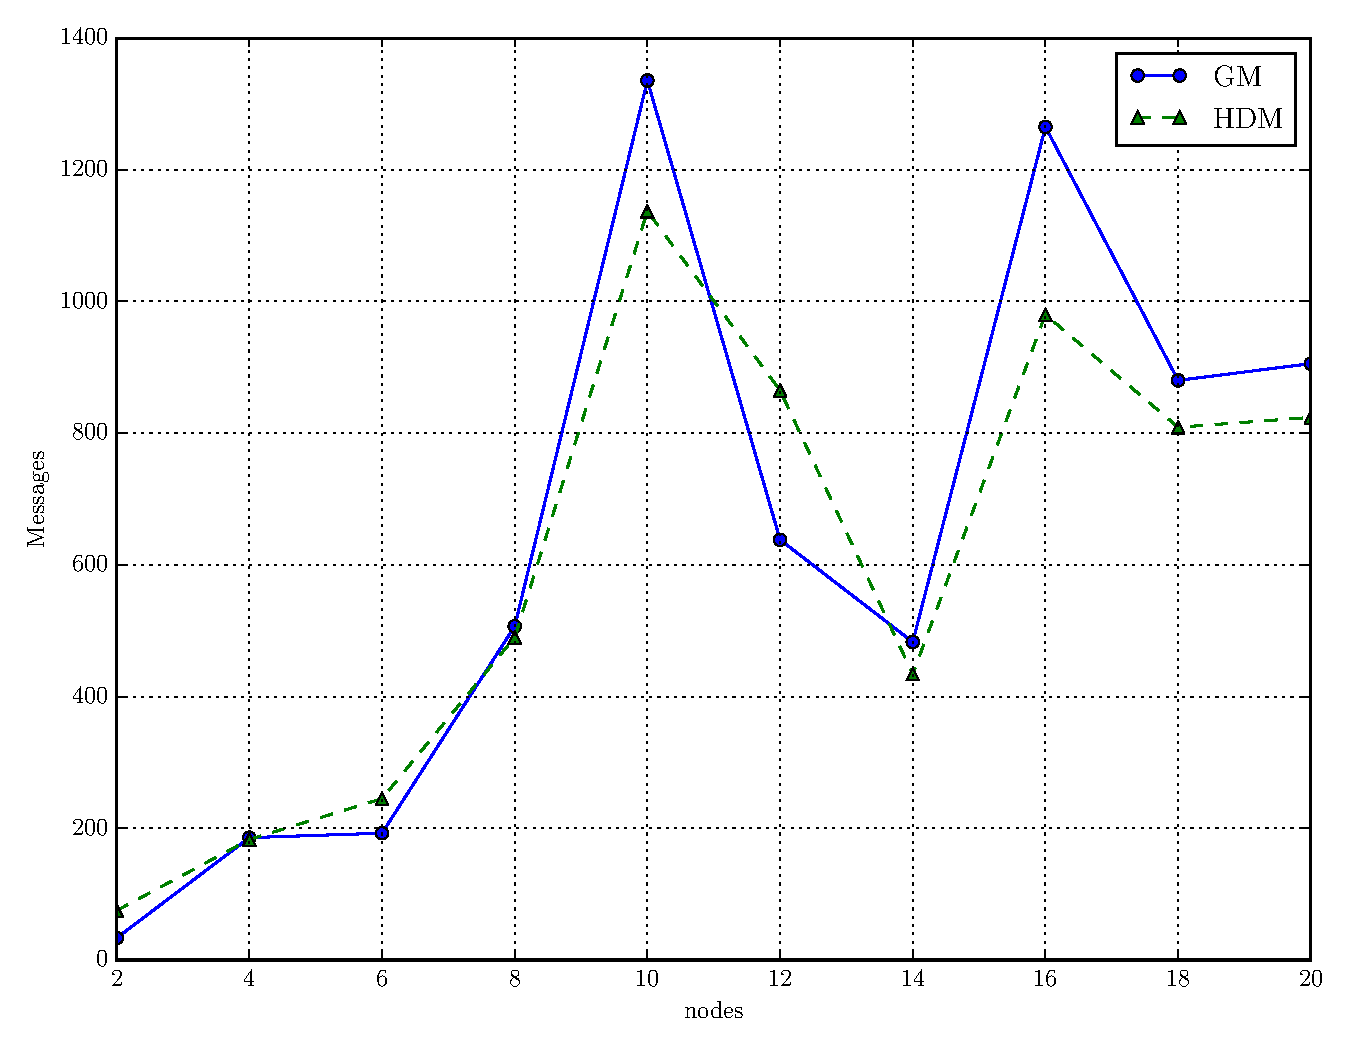
\includegraphics[scale=0.3]{../img/main_msg_interweaving_nodes.pdf}
  \caption{Communication cost of methods GM and HDM for the \emph{INT} dataset.}
\end{figure}
\end{frame}

\begin{frame} \frametitle{GM, HDM Comparison}\framesubtitle{\emph{NOISE}}
\begin{figure}
\vspace{-0.5cm}
\centering
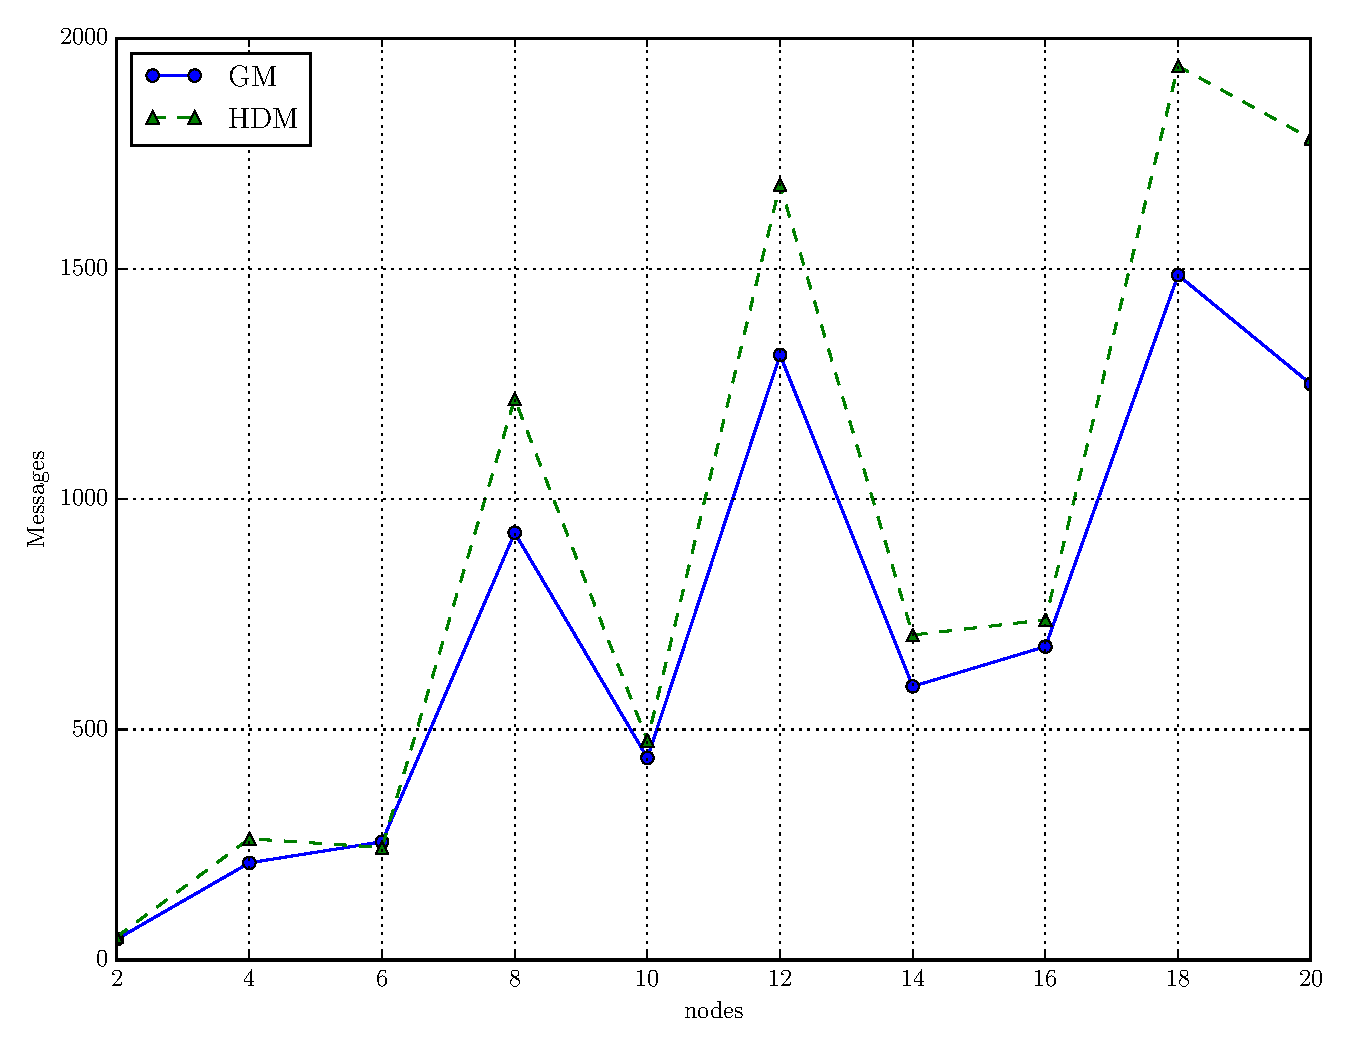
\includegraphics[scale=0.3]{../img/main_msg_noisyinterweaving_nodes.pdf}
  \caption{Communication cost of methods GM and HDM for the \emph{NOISE} dataset.}
\end{figure}
\end{frame}


\begin{frame} \frametitle{GM, HDM Comparison}\framesubtitle{\emph{NOISE} - window}
\begin{figure}
\vspace{-0.5cm}
\centering
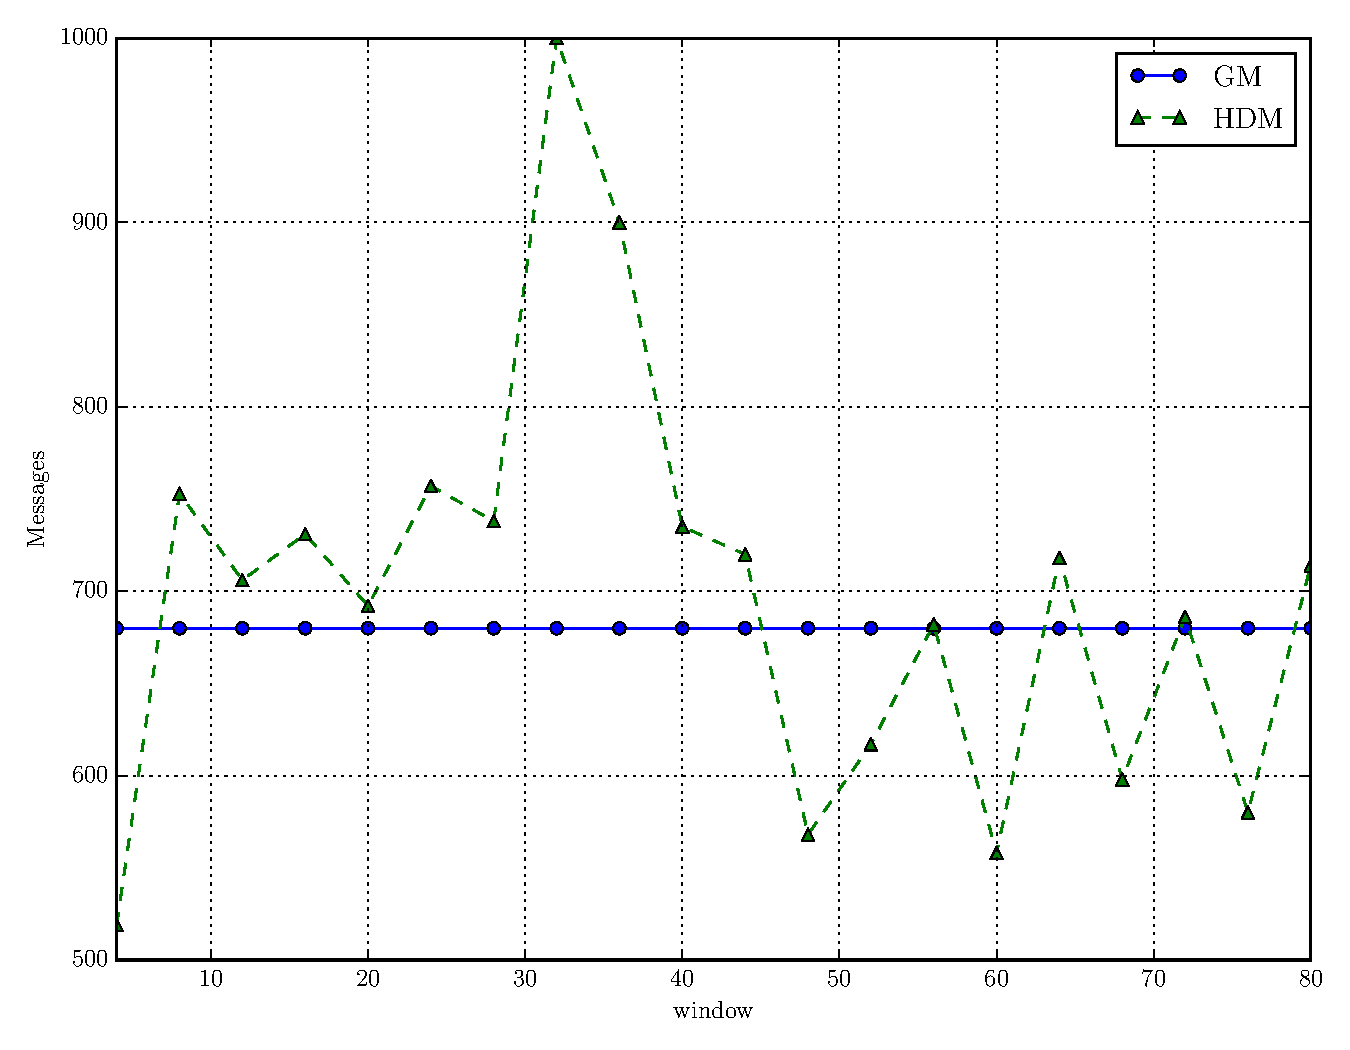
\includegraphics[scale=0.3]{../img/main_msg_noisyinterweaving_window.pdf}
  \caption{Communication cost of methods GM and HDM for the \emph{NOISE} dataset. Approximation order is set to 1.}
\end{figure}
\end{frame}


\begin{frame} \frametitle{GM, HDM Comparison}\framesubtitle{\emph{NOISE} - order}
\begin{figure}
\vspace{-0.5cm}
\centering
 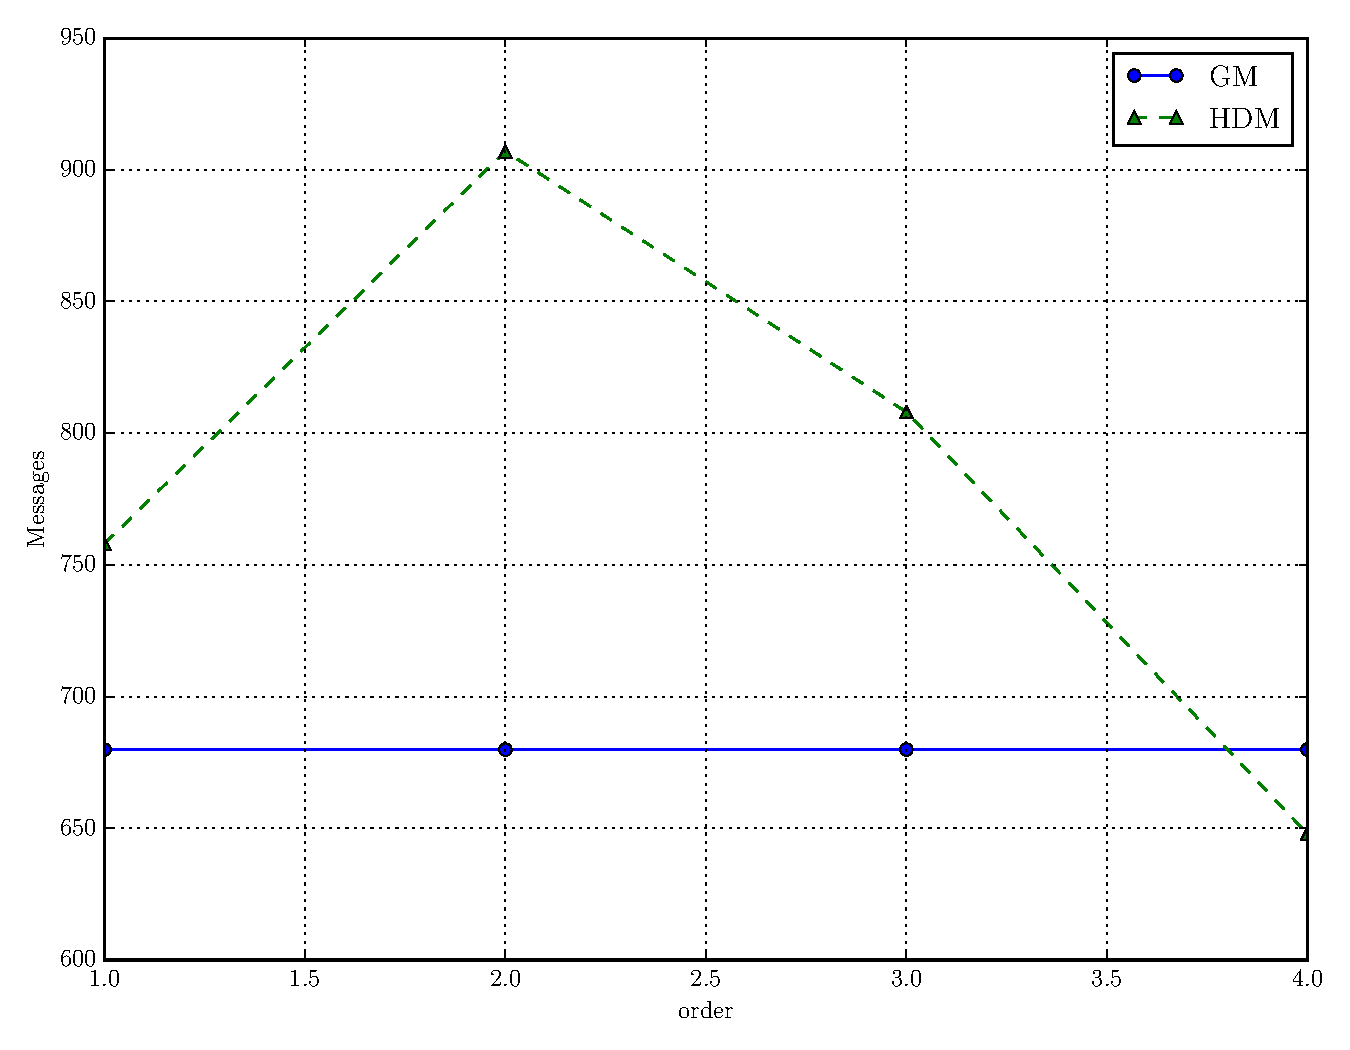
\includegraphics[scale=0.3]{../img/main_msg_noisyinterweaving_order.pdf}
  \caption{Communication cost of methods GM and HDM for the \emph{NOISE} dataset. The Savitzky-Golay window size is set to 24.}
\end{figure}
 \end{frame}

\begin{frame} \frametitle{GM, HDM Comparison}\framesubtitle{Dimensions - Quadratic Function}
\begin{columns}
\begin{column}[t]{0.5\linewidth}
\begin{figure}
\vspace{-1cm}
\centering
  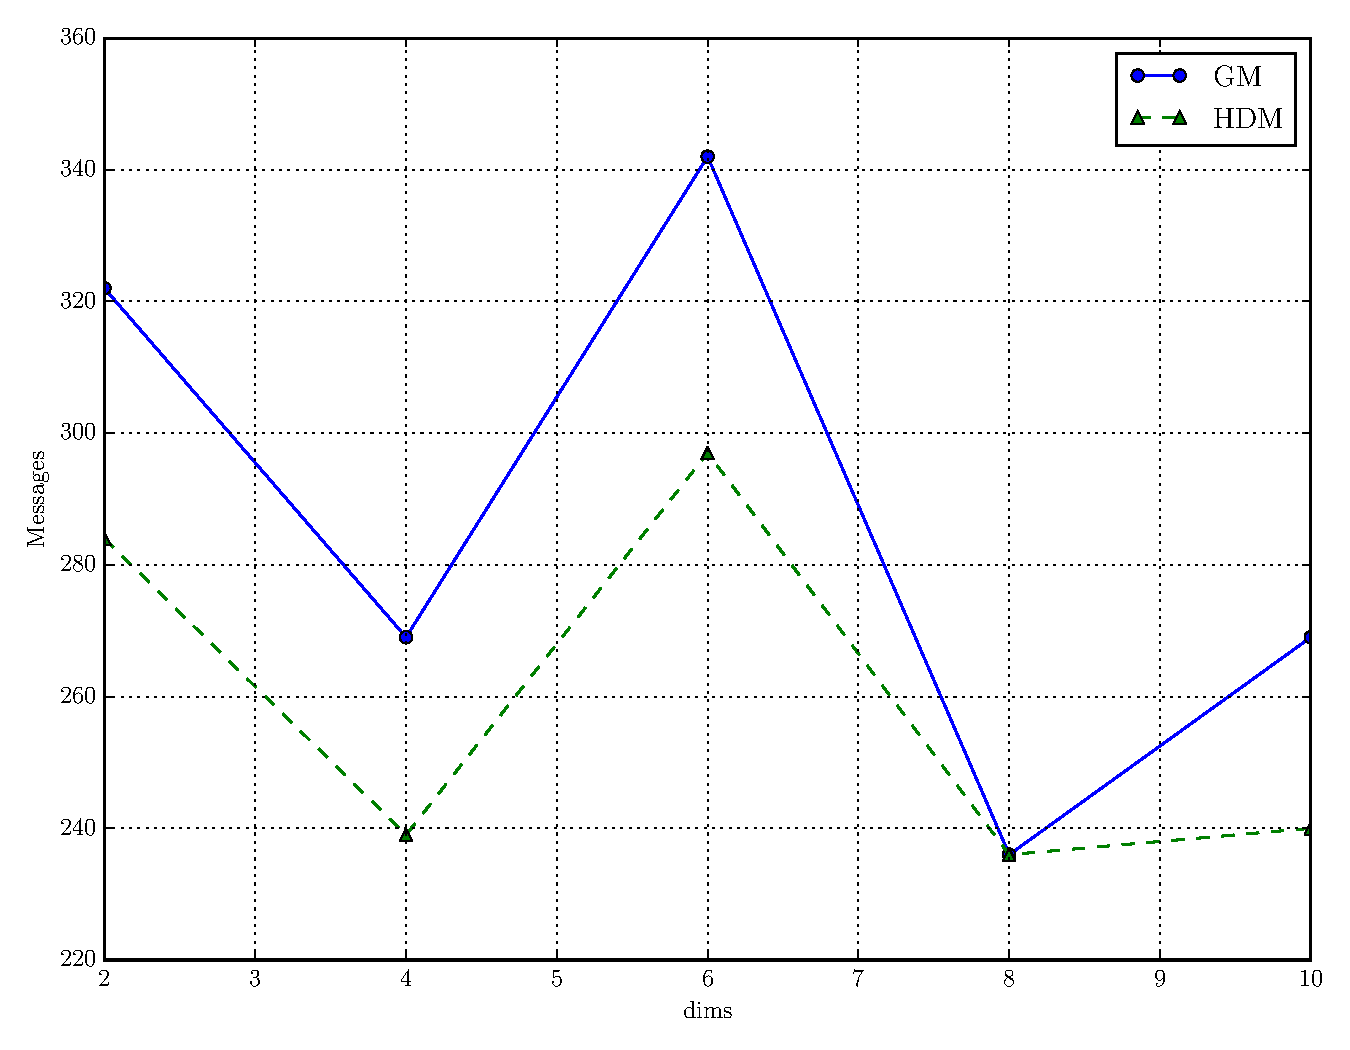
\includegraphics[scale=0.25]{../img/main_msg_linear_dims.pdf}
  \caption{Communication cost of methods GM and HDM for the \emph{LIN} dataset.}
\end{figure}
\end{column}
\begin{column}[t]{0.5\linewidth}
\begin{figure}
\vspace{-1cm}
\centering
  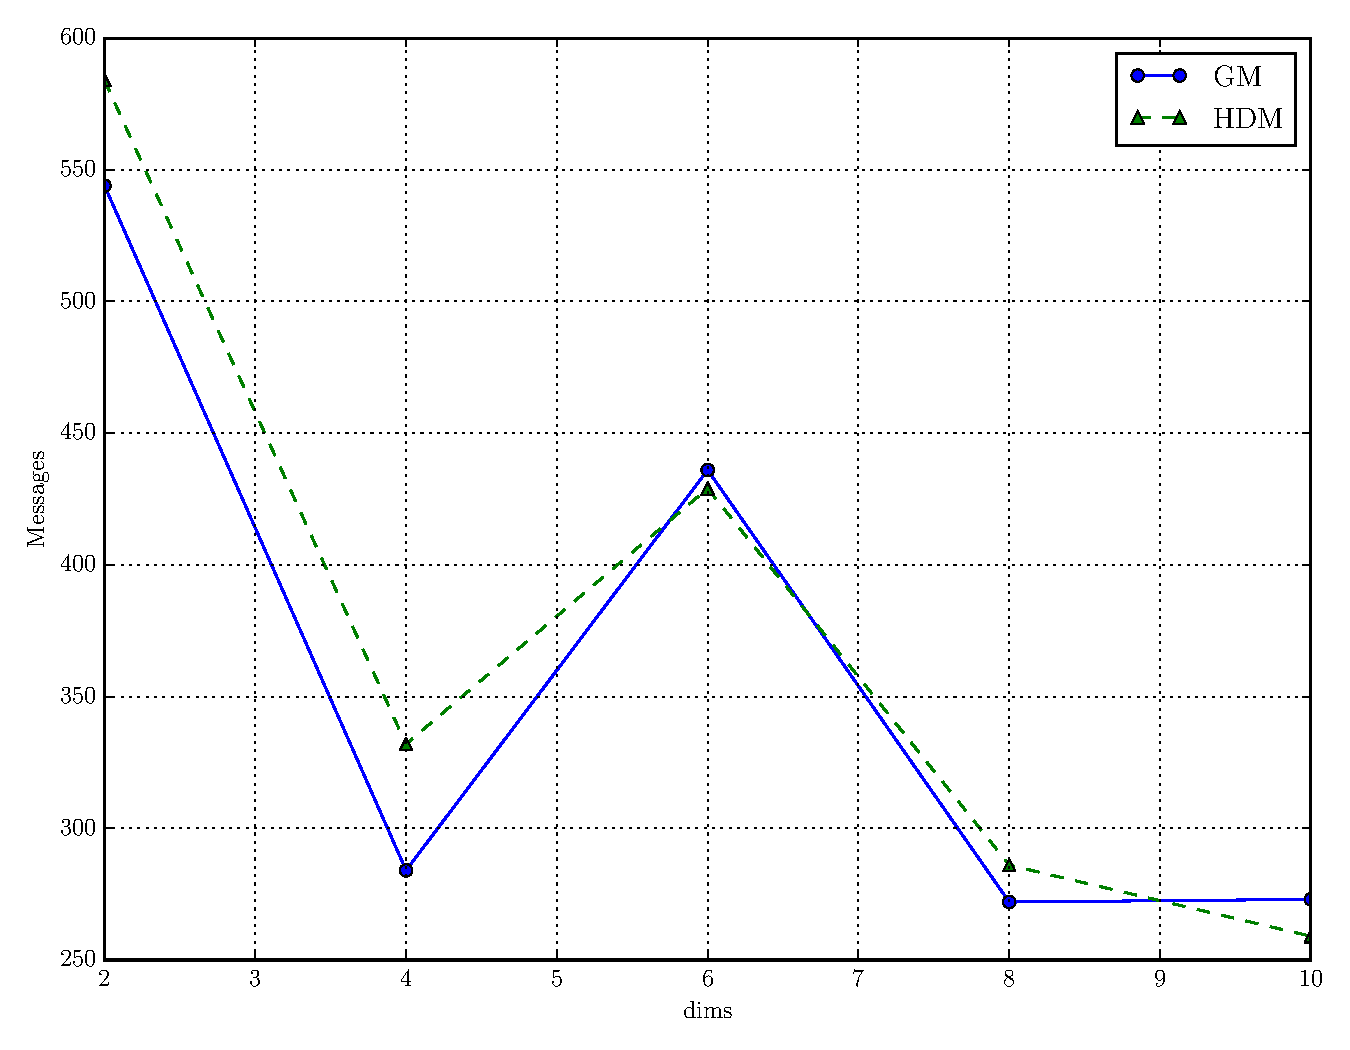
\includegraphics[scale=0.25]{../img/main_msg_noisyinterweaving_dims.pdf}
  \caption{Communication cost of methods GM and HM for the \emph{NOISE} dataset.}
\end{figure}
\end{column}
\end{columns}
\end{frame}
 
\subsubsection*{Real-world Data}
\begin{frame} \frametitle{GM, HDM Comparison}\framesubtitle{Air Pollution Monitoring}
\begin{columns}
\begin{column}[t]{0.5\linewidth}
\begin{figure}
\vspace{-0.8cm}
\centering
   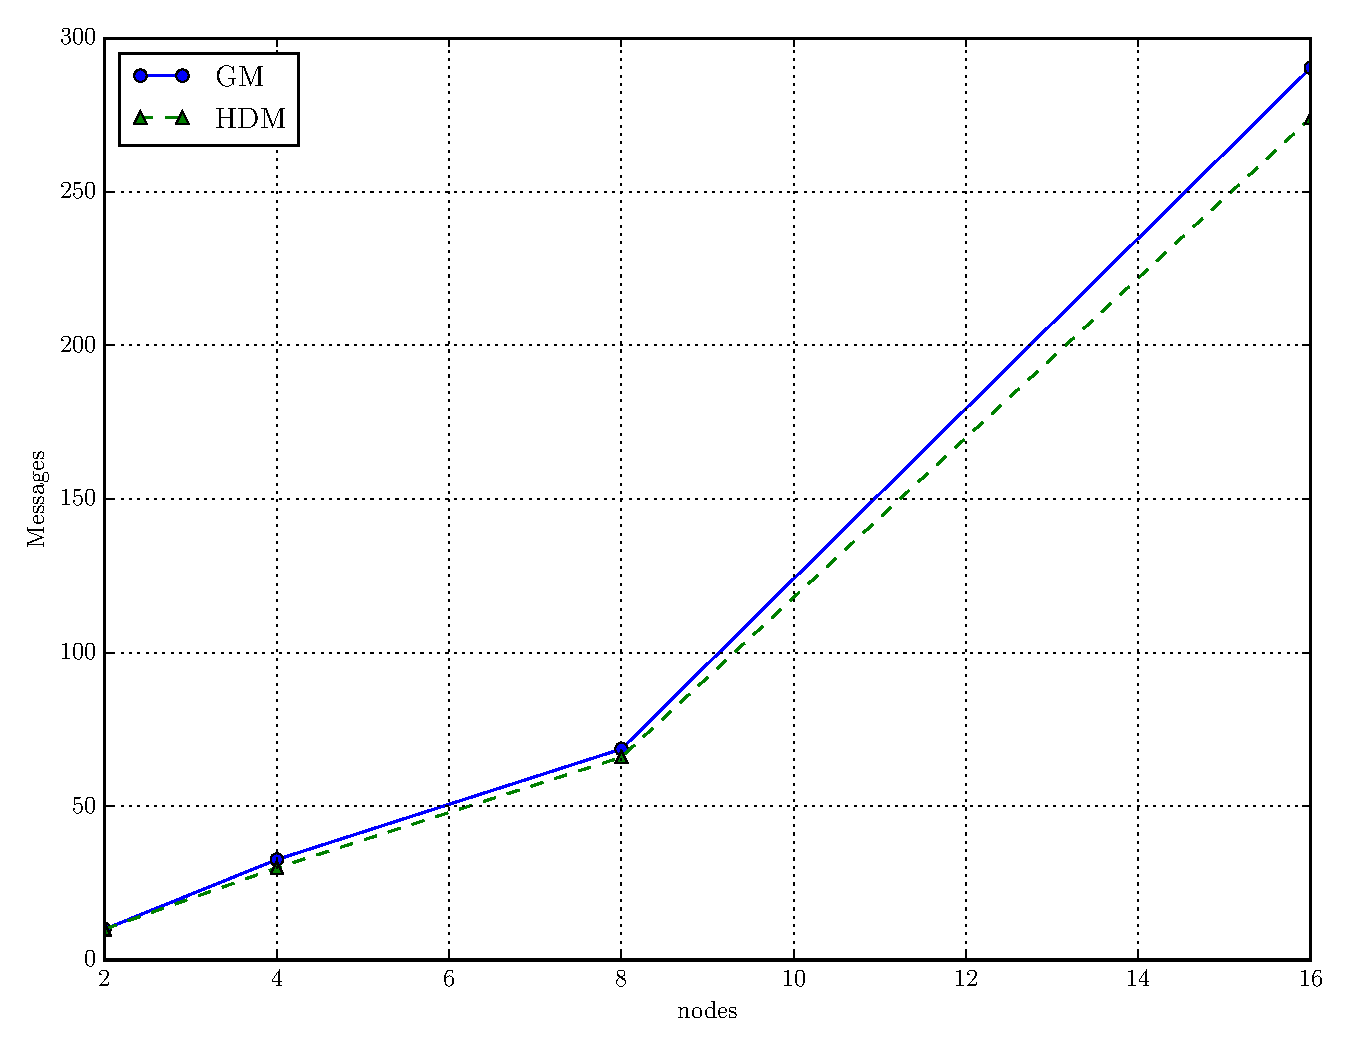
\includegraphics[scale=0.23]{../img/actual_msg_NO2_sq_2014_nodes_wl_6_order_2.pdf}
  \caption{4 to 16 nodes,variance monitoring of $NO_2$. The Savitzky-Golay window size is set to 6, the order is set to 2.}
\end{figure}
\end{column}
\begin{column}[t]{0.5\linewidth}
\begin{figure}
\vspace{-0.8cm}
\centering
  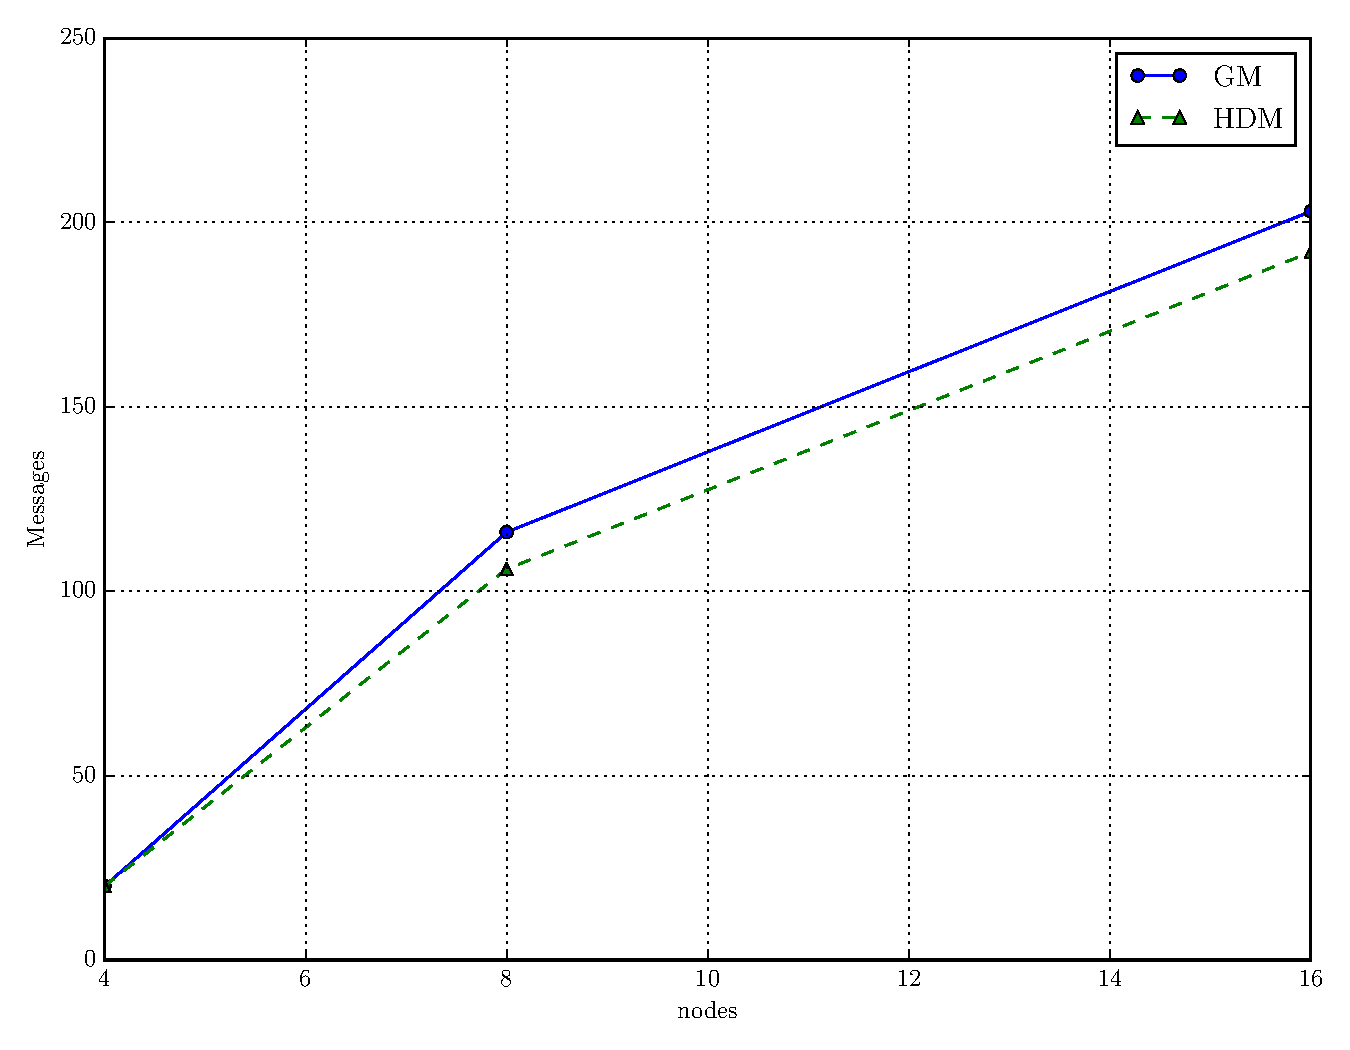
\includegraphics[scale=0.23]{../img/actual_msg_NO2_NO_2014_nodes.pdf}
  \caption{4 to 16 nodes, when monitoring $NO/NO_2$. The Savitzky-Golay window size is set to 10, the order is set to 1.}
\end{figure}
\end{column}
\end{columns}
\end{frame}
%%%%%%%%%%%%%  section: CONCLUSION  %%%%%%%%%%%%%%%%%%%%%%%
\section{Conclusions \& Future Work}
\begin{frame}
  \tableofcontents[currentsection]
\end{frame}

\subsection{Conclusion}
\begin{frame} \frametitle{Summary \& Concluding Remarks}
The \emph{Geometric monitoring} method:
\begin{itemize}
\item An efficient framework for monitoring distributed data streams
\item Scalability can be improved $\rightarrow$ reduce communication costs
\end{itemize}
Our contributions:
\begin{itemize}
\item Distance-based hierarchical node clustering
\item Heuristic balancing method based on SQP and Savitzky-Golay Filtering
\item Detailed evaluation of proposed methods
\end{itemize}
Comments:
\begin{itemize}
\item[+] Communication reduction of up to 60\%
\item[+] Methods fully compatible with the rest of the work
\item[-] Parameter tweaking for satisfactory results
\item[-] Multi-objective optimization can be computationally expensive
\end{itemize}
\end{frame}

\subsection{Future Work}
\begin{frame} \frametitle{Future Work}
\begin{itemize}
\item Multi-objective optimization solvers
\item More elaborate optimizing fuctions
\item Sophisticated prediction models (Gaussian processes)
\item Parameter estimation techniques
\end{itemize}
\end{frame}

\begin{frame}[plain]\frametitle{The End}
\centering
\Huge
Thank you\\
Questions?
\end{frame}



%\begin{frame} \frametitle{System Architecture} \framesubtitle{Decentralized Scenario}
%\begin{figure}[H]
%\centering
%\vspace{-0.2cm}
%\includegraphics[scale=0.5]{../img/decentralized.tex}
%\caption{\textbf{Mesh-like network topology} example of the decentralized scenario. Dashed lines represent data streams and half arrows represent message exchanges.} 
%\end{figure}
%\end{frame}

%\begin{frame} \frametitle{Geometric Interpretation}\framesubtitle{Convexity Property}
%\begin{theorem}[\footfullcite{Sharfman2006GM}]\label{theorem:convexHull}
%Let $\vec{x}, \vec{y_1}, \dots, \vec{y_n} \in \mathbb{R}^d$ be a set of vectors in $\mathbb{R}^d$. Let $Conv(\vec{x}, \vec{y_1}, \dots, \vec{y_n})$ be the convex hull of $\vec{x}, \vec{y_1}, \dots, \vec{y_n}$. Let $B(\vec{x}, \vec{y_i})$ be a ball centered at $\frac{\vec{x}+\vec{y_i}}{2}$ and with radius of $\lVert{\frac{\vec{x}+\vec{y_i}}{2}}\rVert_2$ i.e., $B(\vec{x}, \vec{y_i})=\{\vec{z}\ |\ \lVert{\vec{z}-\frac{\vec{x}+\vec{y_i}}{2}}\rVert_2 \leq \lVert{\frac{\vec{x}+\vec{y_i}}{2}}\rVert_2 \}$, then $Conv(vec{x}, \vec{y_1}, \dots, \vec{y_n}) \subset B(\vec{x}, \vec{y_i})$.
%\end{theorem}
%\end{frame}


%\begin{frame}[plain] \frametitle{Protocol}\framesubtitle{Decentralized Algorithm}
%
%\hfill    \scalebox{0.50}{
%    \begin{minipage}{\linewidth}
%\vspace{-2cm}    
%    \begin{algorithm}[H]
%\setstretch{1.30}
%
%
%\Begin{
%	\ForEach(\tcc*[f]{Node initialization}){node $p_i$}{
%		Broadcast $\vec{v_i}(0)$\;
%		$\vec{v_i}'=\vec{v_i}(0)$\;
%		Wait messages from all other nodes\;
%		\If{messages from all vectors received}{
%			Compute \emph{estimate vector} $\vec{e}(t)$\;
%		}
%	}
%	\ForEach(\tcc*[f]{Main monitoring task}){node $p_i$}{
%		\ForEach{new $s_i$ stream update $\vec{v_i}(t)$}{
%			Recalculate \emph{drift vector} $\vec{u_i}(t)$\;
%			\If{$B(\vec{e},\vec{u_i}(t))$ is \emph{not} monochromatic}{
%				Broadcast message $<i,\vec{v_i}(t)>$\;
%				Set $\vec{v_i}'=\vec{v_i}(t)$\;
%			}
%			\If{new message $<j,\vec{v_j}(t)>$ received}{
%				Set $\vec{v_j}'=\vec{v_j}(t)$\;
%				Recalculate \emph{estimate vector} $\vec{e}(t)$\;
%				\If{$B(\vec{e},\vec{u_i}(t))$ is \emph{not} monochromatic}{
%					Broadcast message $<i,\vec{v_i}(t)>$\;
%					Set $\vec{v_i}'=\vec{v_i}(t)$\;
%				}
%			}
%		}
%	}
%}
%\caption{Decentralized algorithm \label{algo:decentralized}} 
%\end{algorithm}  
%\end{minipage}%
%    }
%\end{frame}

%
%\begin{frame}[plain] \frametitle{Protocol}\framesubtitle{Centralized Algorithm}
%\noindent\scalebox{0.44}{
%\begin{minipage}{\linewidth}
%\hspace{-2cm}
%\begin{algorithm}[H]
%\setstretch{1.30}
%
%\SetKwFunction{Balance}{Balance}
%\SetKwProg{Fn}{Function}{}{end}
%
%\Begin{
%	
%	Wait for $<INIT, \cdot>$ messages from all monitoring nodes\tcc*[r]{Initialization}
%	Compute \emph{estimate vector} $\vec{e}(0)$\;
%	\If(\tcc*[f]{Monitoring operation}){new $<REP,\vec{v_i}(t),\vec{u_i}(t)>$ message received}{
%		$P'=P' \cup \{<i,\vec{v_i}(t),\vec{u_i}(t)>\}$\;
%		\Balance{$P'$}\;
%	}
%}
%\Fn(\tcc*[f]{Balancing Process}){\Balance{$P'$}}{
%	Compute \emph{balancing vector} $\vec{b}$\;
%	\uIf{$B(\vec{e}, \vec{b})$ is \emph{not} monochromatic}{
%		\uIf{$P-P'\neq \emptyset$}{
%			Send $<REQ>$ message to random node in $P-P'$ set\;
%		}
%		\Else{
%			Compute \emph{estimate vector} $\vec{e}(t)$\;
%			Send $<NEW\textnormal{-}EST, \vec{e}(t)>$ message to all nodes\;
%			\Return \;
%		}
%	}
%	\Else{
%		\ForEach{$p_i \in P'$}{
%			Compute \emph{slack adjustment vector} $\Delta\vec{\delta_i}$\;
%			Send $<ADJ\textnormal{-}SLK, \Delta\vec{\delta_i}>$ message to node $p_i$\;
%			\Return \;
%		}
%	}
%
%}
%\caption{Centralized algorithm's coordinator node operation\label{algo:centralizedCoordinatorNode}} 
%\end{algorithm}
%
%\end{minipage}%
%}\hfill\noindent\scalebox{0.42}{
%\begin{minipage}{\linewidth}
%\vspace{-2.5cm}
%\begin{algorithm}[H]
%\setstretch{1.30}
%\Begin{
%	\ForEach(\tcc*[f]{Node initialization}){node $p_i$}{
%		Send $<INIT,\vec{v_i}(0)>$ message to coordinator\;
%		$\vec{v_i}'=\vec{v_i}(0)$\;
%		$\vec{\delta_i}=\vec{0}$\;
%		Wait message from coordinator\;
%		\If{$<NEW\textnormal{-}EST, \vec{e}>$ message received}{
%			Set $\vec{e}(t)=\vec{e}$\;
%		}
%	}
%
%	\ForEach(\tcc*[f]{Main monitoring task}){node $p_i$}{
%		\ForEach{new $s_i$ stream update $\vec{v_i}(t)$}{
%			Recalculate \emph{drift vector} $\vec{u_i}(t)$\;
%			\If{$B(\vec{e},\vec{u_i}(t))$ is \emph{not} monochromatic}{
%				Send $<REP,\vec{v_i}(t),\vec{u_i}(t)>$ message to coordinator\;
%				Wait for $<NEW\textnormal{-}EST,\cdot>$ or $<ADJ\textnormal{-}SLK,\cdot>$ message from coordinator\;
%			}
%		
%		
%			\If{new message $<REQ>$ received}{
%				Send $<REP,\vec{v_i}(t),\vec{u_i}(t)>$ message to coordinator\;
%				Wait for $<NEW\textnormal{-}EST,\cdot>$ or $<ADJ\textnormal{-}SLK,\cdot>$ message from coordinator\;
%
%			}
%
%			\If{new $<NEW\textnormal{-}EST, \vec{e}>$ message received}{
%				Set $\vec{e}(t)=\vec{e}$\;
%				$\vec{v_i}'=\vec{v_i}(t)$\;
%				$\vec{\delta_i}=\vec{0}$\;
%			} 
%
%			\If{new $<ADJ\textnormal{-}SLK, \Delta\vec{\delta_i}>$ message received}{
%				Recompute \emph{delta vector} $\vec{\delta_i}$\;
%			}
%		}
%	}
%}
%\caption{Centralized algorithm's monitoring node operation \label{algo:centralizedMonitoringNode}} 
%\end{algorithm}
%\end{minipage}%
%}
%\end{frame}


%\begin{frame} \frametitle{Non-linear Constraint Optimization}\framesubtitle{Primal Descent}
%\centering
%\scalebox{0.75}{
%\begin{minipage}{1.3\linewidth}
%\begin{algorithm}[H]
%\setstretch{1.30}
%\Begin{
%	Choose initial point $x_0 \in X$ and set $t=0$ \tcc*[r]{Initialization}
%	\While(\tcc*[f]{Search}){maximum iteration limit \emph{OR} convergence}{
%		$t=t+1$\;
%		Determine search direction $d_t$\;
%		Determine step length $s_t$, so that $f(x_t+s_td_t)<f(x_t)$\;
%		Update\;
%	}
%}
%\caption{Generic primal descent \label{algo:nco-primal_descent}} 
%\end{algorithm}
%\end{minipage}%
%}
%\end{frame}

%%conmin
%\begin{frame} \frametitle{Feasible Directions}
%\emph{Usable feasible direction} $d_t$:\begin{itemize}
%\item a small disposition towards direction $d_t$ does not violate any constraint i.e.,
%$$d_t^T \nabla G(x_t)\leq 0$$
%\item a move towards $d_t$ reduces the objective functions value i.e.,
%$$d_t^T \nabla F(x_t)<0$$.
%\end{itemize}
%\end{frame}

%\begin{frame}
%\scalebox{0.50}{
%\begin{minipage}[t]{\linewidth}
%\begin{algorithm}[H]
%\setstretch{1.30}
%
%\KwData{$monitoringNodes$: a list of Monitoring nodes,\\\quad $coordinator$: the Coordinator node}
%
%\SetAlgoLined
%\Begin{
% initialization\;
% 	\Repeat{$globalViolation$}{
%		\ForEach{$node \in\ monitoringNodes$}{
%			$node.DataVectorUpdate()$\;
%			$node.ComputeDriftVector()$\;
%		}
%		\ForEach{$node \in\ monitoringNodes$}{
%			$node.CheckForViolation()$\;
%			\If{$localViolation$}{
%				$node.Report()$\;
%				$coordinator.Balance()$\;
%			}
%		}
%	}
%}
%\caption{Iterative network operation \label{algo:singleHandlingNetwork}} 
%\end{algorithm}
%\end{minipage}%
%}
%\end{frame}


%\begin{frame}[plain] \frametitle{The Distance-based Hierarchical Clustering}\framesubtitle{The Algorithm}
%\centering
%\scalebox{0.70}{
%\begin{minipage}[t]{1.3\linewidth}
%\begin{algorithm}[H]
%\SetAlgoLined
%\setstretch{1.30}
%\SetKwFunction{DistancePairer}{DistancePairer}
%\SetKwProg{Fn}{Function}{}{end}
%\Fn{\DistancePairer{$nodes$,$i$}}{
%	\KwData{$nodes=[(n_1, [\vec{v_1}(t_0), ... , \vec{v_1}(t_{end})]), ... , (n_k, [\vec{v_k}(t_0), ... , \vec{v_k}(t_{end})])]$: list of nodes with their respective data vectors,$i$: pair type, initial=1} 
%	\KwResult{$nodeHierarchy$: dictionary of \emph{Type-k} pairs}
%
%	\If(\tcp*[f]{recursion stopping condition}){$length(nodes)=1$}{
%		\Return{$nodeHierarchy$}\;
%	}
%	$g=CreateCompleteGraph(nodes)$\tcp*[r]{complete graph with $nodes$ as vertices} 
%	\ForEach(\tcp*[f]{assign weights to edges}){$(n_i, n_j)\in g.Edges()$}{
%		$w_{i,j}=
%		\sum_{t=t_0}^{t_{end}}{[(f(\vec{v}_{global}(t))-f(\frac{\vec{v_i}(t)+\vec{v_j}(t)}{2}))+(|\vec{v_i}(t)-\vec{v_j}(t)|)]}$\;
%		$g.edge(n_i, n_j).weight=w_{i,j}$\;
%	}
%	$nodeHierarchy(\text{Type-i})=g.maximalWeightMatching()$\tcp*[r]{node pairs of \emph{Type-}$i$}
%	\DistancePairer{$nodeHierarchy(\text{Type-i}),i*2$}\;
%}
%\caption{Recursively create Monitoring node pairs and hierarchy \label{algo:nodeMatching}} 
%\end{algorithm}
%\end{minipage}
%}
%\end{frame}


%\begin{frame} \frametitle{The Heuristic Balancing}\framesubtitle{The Function Implementation}
%\begin{align*}
%\min -z&\\
%	\text{s.t.}\ \ z&\leq g(h(\vec{e},\vec{u_0}), vel_0, accel_0, T)\\
%	z&\leq g(h(\vec{e},\vec{u_1}), vel_1, accel_1, T)\\
%	&\vdots \\
%	z&\leq g(h(\vec{e},\vec{u_n}), vel_n, accel_n, T)\\
%	\vec{b}&=\frac{1}{\sum_{i=0}^n{w_i}}\sum_{i=0}^n{(w_i*\vec{u_i})} &&,\forall n_i \in P'
%\end{align*}
%where:
%\begin{align*}
%g&:\mathbb{R}^4 \to \mathbb{R}, \text{the heuristic optimization function as defined in Equation~\ref{form:heuristic}}\\
%h&:\mathbb{R}^d \to \mathbb{R}, \text{the function computing the maximum value of the monitoring function $f(\cdot)$ in $B(\vec{e},\vec{u_i})$,}\\&\qquad\text{which is an optimization problem by itself}\\
%d&: \text{the data vector dimensionality}
%\end{align*}
%\end{frame}
%
%\begin{frame}[plain] \frametitle{The Heuristic Balancing}\framesubtitle{The Algorithm}
%\centering
%\scalebox{0.65}{
%\begin{minipage}[t]{1.5\linewidth}
%\begin{algorithm}[H]
%\SetAlgoLined
%\setstretch{1.30}
%\SetKwFunction{RepMessageReceived}{RepMessageReceived}
%\SetKwFunction{RequestNode}{RequestNode}
%\SetKwFunction{Balance}{Balance}
%\SetKwProg{Fn}{Function}{}{end}
%
%\Fn{\RepMessageReceived{$<n_i$,$v_i$,$u_i$,$vel_i$,$accel_i>$}}{
%	add $n_i$ to balancing set $P'$\;
%	\Balance{}\;
%}
%
%\Fn{\Balance{$P'$}}{
%	\If{$length(P')=1$}{
%		\RequestNode{}\tcp*[r]{request node based on respective gathering scheme}
%	}
%
%	$\vec{b}=\sum_{P'}{\frac{w_i*\vec{u_i}}{w_i}}$\;
%
%	\If{$B(\vec{e},\vec{b})$ is monochromatic}{
%		\tcc{heuristic optimization procedure,\\ returns the optimal drift vector positions in set $O$}
%		$O=DriftVectorOptimizationProblem()$\;
%
%		\ForEach{$n_i \in P'$}{
%			$\Delta\delta_i=w_i*\vec{u_i}'-w_i*\vec{u_i}$\tcp*[r]{$\vec{u_i}'$ denotes the optimal drift vector position}
%			$Send(<ADJSLK,n_i,\Delta\delta_i>)$\;
%		}
%	}
%}
%\caption{Heuristic Balancing \label{algo:heuristicbalancing}} 
%\end{algorithm}
%\end{minipage}
%}
%\end{frame}

\end{document}

